\documentclass[12pt, twoside, openright]{report} %fuente a 12pt, formato doble pagina y chapter a la derecha
\raggedbottom % No ajustar el contenido con un salto de pagina

% MÁRGENES: 2,5 cm sup. e inf.; 3 cm izdo. y dcho.
\usepackage[
a4paper,
vmargin=2.5cm,
hmargin=3cm
]{geometry}

% INTERLINEADO: Estrecho (6 ptos./interlineado 1,15) o Moderado (6 ptos./interlineado 1,5)
\renewcommand{\baselinestretch}{1.15}
\parskip=6pt

% DEFINICIÓN DE COLORES para portada y listados de código
\usepackage[table]{xcolor}
\definecolor{azulUC3M}{RGB}{0,0,102}
\definecolor{gray97}{gray}{.97}
\definecolor{gray75}{gray}{.75}
\definecolor{gray45}{gray}{.45}

% Soporte para GENERAR PDF/A
\usepackage[a-1b]{pdfx}

% ENLACES
\usepackage{hyperref}
\hypersetup{colorlinks=true,
	linkcolor=black, % enlaces a partes del documento (p.e. índice) en color negro
	urlcolor=blue} % enlaces a recursos fuera del documento en azul

% Añadir pdfs como partes del documento
\usepackage{pdfpages}

% Quitar la indentación de principio de los parrafos
\setlength{\parindent}{0em}

% EXPRESIONES MATEMATICAS
\usepackage{amsmath,amssymb,amsfonts,amsthm}

\usepackage{txfonts} 
\usepackage[T1]{fontenc}
\usepackage[utf8]{inputenc}

% Insertar graficas y fotos
\usepackage{tikz}
\usepackage{pgfplots}

\usepackage[spanish, es-tabla]{babel} 
\usepackage[babel, spanish=spanish]{csquotes}
\AtBeginEnvironment{quote}{\small}

% diseño de PIE DE PÁGINA
\usepackage{fancyhdr}
\pagestyle{fancy}
\fancyhf{}
\renewcommand{\headrulewidth}{0pt}
\fancyfoot[LE,RO]{\thepage}
\fancypagestyle{plain}{\pagestyle{fancy}}

% DISEÑO DE LOS TÍTULOS de las partes del trabajo (capítulos y epígrafes o subcapítulos)
\usepackage{titlesec}
\usepackage{titletoc}
\titleformat{\chapter}[block]
{\large\bfseries\filcenter}
{\thechapter.}
{5pt}
{\MakeUppercase}
{}
\titlespacing{\chapter}{0pt}{0pt}{*3}
\titlecontents{chapter}
[0pt]                                               
{}
{\contentsmargin{0pt}\thecontentslabel.\enspace\uppercase}
{\contentsmargin{0pt}\uppercase}                        
{\titlerule*[.7pc]{.}\contentspage}                 

\titleformat{\section}
{\bfseries}
{\thesection.}
{5pt}
{}
\titlecontents{section}
[5pt]                                               
{}
{\contentsmargin{0pt}\thecontentslabel.\enspace}
{\contentsmargin{0pt}}
{\titlerule*[.7pc]{.}\contentspage}

\titleformat{\subsection}
{\normalsize\bfseries}
{\thesubsection.}
{5pt}
{}
\titlecontents{subsection}
[10pt]                                               
{}
{\contentsmargin{0pt}                          
	\thecontentslabel.\enspace}
{\contentsmargin{0pt}}                        
{\titlerule*[.7pc]{.}\contentspage}  


% DISEÑO DE TABLAS.
\usepackage{multirow} % permite combinar celdas 
\usepackage{caption} % para personalizar el título de tablas y figuras
\usepackage{floatrow} % utilizamos este paquete y sus macros \ttabbox y \ffigbox para alinear los nombres de tablas y figuras de acuerdo con el estilo definido. Para su uso ver archivo de ejemplo 
\usepackage{array} % con este paquete podemos definir en la siguiente línea un nuevo tipo de columna para tablas: ancho personalizado y contenido centrado
\newcolumntype{P}[1]{>{\centering\arraybackslash}p{#1}}
\DeclareCaptionFormat{upper}{#1#2\uppercase{#3}\par}

% Diseño de tabla para ingeniería
\captionsetup[table]{
	format=hang,
	name=Tabla,
	justification=centering,
	labelsep=colon,
	width=.75\linewidth,
	labelfont=small,
	font=small,
}

% DISEÑO DE FIGURAS.
\usepackage{graphicx}
\graphicspath{{img/}} %ruta a la carpeta de imágenes

% Diseño de figuras para ingeniería
\captionsetup[figure]{
	format=hang,
	name=Fig.,
	singlelinecheck=off,
	labelsep=colon,
	labelfont=small,
	font=small		
}

% NOTAS A PIE DE PÁGINA
\usepackage{chngcntr} %para numeración continua de las notas al pie
\counterwithout{footnote}{chapter}

% LISTADOS DE CÓDIGO
% soporte y estilo para listados de código. Más información en https://es.wikibooks.org/wiki/Manual_de_LaTeX/Listados_de_código/Listados_con_listings
\usepackage{listings}

% definimos un estilo de listings
\lstdefinestyle{estilo}{ frame=Ltb,
	framerule=0pt,
	aboveskip=0.5cm,
	framextopmargin=3pt,
	framexbottommargin=3pt,
	framexleftmargin=0.4cm,
	framesep=0pt,
	rulesep=.4pt,
	backgroundcolor=\color{gray97},
	rulesepcolor=\color{black},
	%
	basicstyle=\ttfamily\footnotesize,
	keywordstyle=\bfseries,
	stringstyle=\ttfamily,
	showstringspaces = false,
	commentstyle=\color{gray45},     
	%
	numbers=left,
	numbersep=15pt,
	numberstyle=\tiny,
	numberfirstline = false,
	breaklines=true,
	xleftmargin=\parindent
}

\captionsetup[lstlisting]{font=small, labelsep=period}
% fijamos el estilo a utilizar 
\lstset{style=estilo}
\renewcommand{\lstlistingname}{\uppercase{Código}}

\pgfplotsset{compat=1.17} 
%-------------
%	DOCUMENTO
%-------------

\begin{document}
\pagenumbering{roman} % Se utilizan cifras romanas en la numeración de las páginas previas al cuerpo del trabajo

%----------
%	PORTADA
%----------	
\begin{titlepage}
	\begin{sffamily}
		\color{azulUC3M}
		\begin{center}
			\begin{figure}[H] %incluimos el logotipo de la Universidad
				\makebox[\textwidth][c]{
\includegraphics[width=16cm]{Portada_Logo.png}}
			\end{figure}
			\vspace{2.5cm}
			\begin{Large}
				Grado en Ingeniería Informática\\
				2020-2021\\
				\vspace{2cm}
				\textsl{Apuntes}\\
				\bigskip
			\end{Large}
			{\Huge Diseño de Sistemas Operativos}\\
			\vspace*{0.5cm}
			\rule{10.5cm}{0.1mm}\\
			\vspace*{0.9cm}
			{\LARGE Jorge Rodríguez Fraile\footnote{\href{mailto:100405951@alumnos.uc3m.es}{Universidad: 100405951@alumnos.uc3m.es}  |  \href{mailto:jrf1616@gmail.com}{Personal: jrf1616@gmail.com}}}\\
			\vspace*{1cm}
		\end{center}
		\vfill
		\color{black}
		
\includegraphics[width=4.2cm]{img/creativecommons.png}\\
		Esta obra se encuentra sujeta a la licencia Creative Commons\\ \textbf{Reconocimiento - No Comercial - Sin Obra Derivada}
	\end{sffamily}
\end{titlepage}

%----------
%	ÍNDICES
%----------	

%--
% Índice general
%-
\tableofcontents
\thispagestyle{fancy}

%--
% Índice de figuras. Si no se incluyen, comenta las líneas siguientes
%-
\listoffigures
\thispagestyle{fancy}

%--
% Índice de tablas. Si no se incluyen, comenta las líneas siguientes
%-
\listoftables
\thispagestyle{fancy}

%----------
%	TRABAJO
%----------	

\pagenumbering{arabic} % numeración con números arábigos para el resto de la publicación	

%----------
%	COMENZAR A ESCRIBIR AQUI
%----------	


\chapter{Información}
\section{Profesores}

\begin{quote}
	Teorías: Javier García Guzmán

	Prácticas: Mat Max Montalvo Martínez
\end{quote}

\chapter{Tema 1: Arquitectura de Sistemas
  IoT}


\textbf{IoT - Internet de las Cosas}: Consiste en conectar a internet
cualquier dispositivo, vehículo, edificios o en general objetos a los
que se les haya dotado de sensores, actuadores y conexión a la red. Lo
que les permite obtener e intercambiar información. Red de objetos
conectados a internet que aporta valor añadido a los usuarios que
interactúan con ellos.

Consiste en añadir \textbf{inteligencia computacional} a dispositivos
para mejorar las funcionalidades.

Permite que los dispositivos puedan intercambiar información.

Se busca que sean pequeños y tengan un chip que les permita
\textbf{conectarse a la red} y operar en ella. Lo estandarizo IBM.

El \textbf{top 6 áreas} de aplicación de IoT:

\begin{enumerate}
	\def\labelenumi{\arabic{enumi}.}
	\item \textbf{Industrial/Fabricación}: Automatizar, controlar la
	      distribución, gestión de instalaciones.
	\item \textbf{Transporte/Movilidad:} Coches, tráfico en ciudad, vehículos de
	      transporte masivo y transporte industrial.
	\item \textbf{Energía/Gestión eléctrica}: Predecir consumo, personalizar,
	      bien estar de los ocupantes, monitorizar el consumo detallado,
	      instalaciones con sensores.
	\item \textbf{Gestión de inventarios/Comercial}: Saber cuánto queda y pedir,
	      facilitar compras.
	\item \textbf{Ciudad}: Recoge muchas áreas; basura, vigilancia, tráfico,
	      etc.
	\item \textbf{Salud:} Investigación, la forma de tratar, las emergencias,
	      distribución de información médica y dispositivos.
\end{enumerate}

\textbf{Agricultura de precisión}: Según las previsiones ambientales y
meteorológicas, plagas y demás se calcula el mejor momento para sembrar.
Además, cuando ya está plantado, las condiciones del suelo, cuando regar
y abonar las tierras, así como la recolecta.

\newpage

\section{En IoT de vehículos hay distintos
  niveles}

\textbf{0}: Sin automatización.

\textbf{1}: Asistencia en la conducción.

\textbf{2}: Control de carril, lateral y longitudinal.

\textbf{3}: Conducción autónoma, pero el conductor en su puesto, para
riesgos.

\textbf{4}: Conducción autónoma, pero el conductor en su puesto,
supervisar.

\textbf{5}: Conducción totalmente autónoma, sin conductor.

\section{Elementos IoT}

\textbf{Colector}: Recogen información, sensores, o se activan,
actuadores, que se intercambian en internet.

\textbf{Transmisor}: Puertas de enlace, pasarelas, pasan los datos a la
red desde los dispositivos.

\textbf{Agregación + Distribución}: Cálculo y procesamiento de la
información.

\textbf{Consumidor}: Los usuarios/clientes acceden a los datos.

\section{Evolución}

3 generaciones.

\begin{enumerate}
	\def\labelenumi{\arabic{enumi}.}
	\item \textbf{RFID y sensores}

	      Tecnología de detección por radiofrecuencia.

	      Las cosas contengan información, las etiquetas (como NFC, se
	      estandarizó para indicar que datos contiene) y tener un dispositivo
	      que al acercarlo podamos leerla.
	\item \textbf{Web services e inter-networking} (2004-2012): Interconexión
	      completa de las cosas y la red de las cosas.

	      IPv4, HTTP, Bluetooth, TCP, UDP, etc.

	      Pasan a tener una manera fácil de conectarse los dispositivos entre sí
	      o con internet.
	\item \textbf{Social, Cloud \& ICN:} La era de la computación en la nube y
	      la Internet del futuro.

	      En esta generación la lógica pasa a estar en la nube, no en el
	      dispositivo.

	      Gestión de grandes cantidades de información.

	      Seguridad, evitar accesos fraudulentos.
\end{enumerate}

\section{Arquitectura de un Sistema IoT}
\begin{description}
	\item[Dispositivos (Devices)] Sensores y actuadores FÍSICOS, que
	      normalmente tienen un microprocesador, que mide el medio físico y
	      transforma las mediciones a señales digitales. Su función es tomar
	      medidas y procesarlas, pero su función no puede ser solo transmitir la
	      información.

	      Actuador, Sensores, LED, LCD, Beacon (la parte dispositivo), Termostato,
	      RFID, Trampa para ratones inteligente, Dispositivos embebidos, etc.
	\item[Pasarela (Gateway)] Dispositivo o protocolo con la capacidad de
	      comunicar con internet los dispositivos, para transmitir los datos
	      tomados. Su única función es transmitir.

	      Router, Wifi, GSM, Bluetooth, Zigbee, Raspberry a veces, AMQP, CoAP,
	      LoRaWAN (sistema de radio), Wimax.

	      Un móvil está entre Device y Gateway.
	\item[Plataforma IoT (IoT Platform)] Conjunto de servicios
	      orquestados para gestionar una gran red de dispositivos interconectados
	      y que proporcionan información a aplicaciones u otros tipos de sistemas
	      de información. Gestiona y almacena grandes cantidades de datos y las
	      redirige. Funciona como middleware.

	      Es una nube de servidores que dan servicios:

	      \begin{enumerate}
		      \item \textbf{Message broker y Message bus}: Se encarga de conectar los
		            dispositivos físicos con los distintos procesos que forman parte de la
		            red de IoT. Manda los datos a todos los que estén conectados a su bus,
		            suscritos por API Rest.
		      \item \textbf{Message router}: Está suscrito al message broker, los mensajes
		            que recibe los enriquece; dando información semántica, de contexto, de
		            estado y los reenvía a aquellos componentes que van a gestionar la
		            lógica de las aplicaciones relacionadas con la nube IoT. Otra cosa que
		            hace es transformar datos, descomprimir y decodificar datos para
		            hacerlos más fáciles de procesar y tratar.
		      \item \textbf{Rest API}: Interfaz que usan otros programas para obtener los
		            servicios o las funcionalidades de un componente. Esta API se
		            caracteriza por ser accesible por http e independiente del estado del
		            sistema.
		      \item \textbf{Data Management}: Para almacenar y gestionar los datos tomados
		            en la red.
		      \item \textbf{Rule engine}: Permite monitorear los mensajes recibidos desde
		            el router y permite lanzar distintas acciones en distintos elementos.
		            Decide que acción tomar.

		            Ejem: Si se abre la puerta, entonces avisar de intruso.
		      \item \textbf{Microservicios}: Proporciona funcionalidades muy específicas a
		            través de una interfaz API Rest bien definidas mediante un contrato de
		            datos. Muchos los coordina el rule engine. Se busca que esté muy
		            cohesionado y poco acoplado.

		            Ejem: El que actualiza la estación meteorológica en el móvil, es un
		            proceso muy concreto.
		      \item \textbf{Device manager}: Permite monitorizar algunos elementos de los
		            sensores físicos como si está activo, la batería o si está conectado a
		            la red.
		      \item \textbf{App y User management}: Sistema de permisos que identifica y
		            gestiona el acceso de usuarios y aplicaciones.
	      \end{enumerate}

	\item[Aplicación (Application)] La interfaz que el usuario utiliza
	      para controlar el sistema.

\end{description}

\textbf{iBeacon} es un ejemplo de protocolo y \textbf{Beacon} es el
dispositivo. Ambos están relacionados con dispositivos.

\textbf{Small Data}: Que solo proporcione la información de valor
añadido. Es un conjunto de datos con un volumen y un formato que hacen
que los datos sean accesibles, informativos y procesables.

\textbf{Wimax}: Conjunto de tecnologías y protocolos para aumentar el
alcance de las redes inalámbricas (en vez de 30 metros, 40 kilómetros).

\chapter{Tema 2: Sensores y
  Actuadores}


Hasta la sección `Up to Functional examples
(putting it all together)' incluida.

\section{Sensores}

Conjunto de componentes electrónicos capaces de detectar cambios físicos
en el entorno y enviar información a otros componentes electrónicos,
generalmente un procesador de computadora.

\textbf{Ejemplos}: Sensor de luz (LDR), sensor de ultrasonidos,
giroscopio, fototransistor, Reed switch, \ldots{}

Los sensores se pueden clasificar en tipos según lo que miden: Gases,
velocidad, flujo, fugas, movimiento, electricidad, \ldots{}

\textbf{Según la señal que produce:}

\begin{itemize}
	\item \textbf{Analógico}: Produce voltaje analógico constante de lo medido.
	      El gráfico de voltaje sobre el tiempo debe ser continuo y suave.

	      \begin{figure}[H]
		      \ffigbox[\FBwidth]
		      {\caption{Diagrama de voltaje Sensor Analógico}}
		      {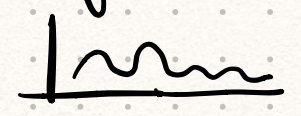
\includegraphics[scale=.5]{image-20210307210139988.png}}
	      \end{figure}
	      \vspace{-0.5cm}
	      Sensor de presión, sensor de luz, sensor de temperatura,
	      acelerómetro, sensor de sonido.
	\item \textbf{Digital}: Produce un voltaje discreto, por lo general tendrá
	      uno u otro de dos valores, 0 V (apagado) a 5 V (encendido). Gracias a la
	      miniaturización hay más dado que se puede introducir un conversor.

	      \begin{figure}[H]
		      \ffigbox[\FBwidth]
		      {\caption{Diagrama de voltaje Sensor Digital}}
		      {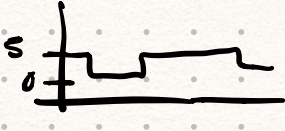
\includegraphics[scale=.5]{image-20210307210421078.png}}
	      \end{figure}
	      \vspace{-0.5cm}
	      Sensor de ultrasonidos, sensor de infrarrojos, acelerómetro, sensor
	      de sonido (suele ser analógico), sensor de temperatura.
\end{itemize}

Según si necesitan energía:

\begin{itemize}
	\item \textbf{Sensor activo}: Siempre \textbf{necesitan} su propia fuente de
	      energía.

	      \begin{itemize}
		      \item Sensor de ultrasonidos, radar, LiDAR, sensor de humedad, cámara
		            infrarroja.
	      \end{itemize}
	\item \textbf{Sensor pasivo}: \textbf{No necesitan} una fuente de energía,
	      usan factores externos para alimentarse.

	      \begin{itemize}
		      \item Sensor infrarrojo (fotodiodo infrarrojo), sensor PIR, sensor de luz
		            (LDR)
	      \end{itemize}
\end{itemize}

\textbf{Sensor piezoeléctrico:}

\begin{enumerate}
	\def\labelenumi{\arabic{enumi}.}
	\item Un cristal piezoeléctrico se coloca entre dos placas de metal que
	      están en perfecto equilibrio y conduce ninguna corriente eléctrica.
	\item Las placas de metal aplican tensión o fuerza mecánica sobre el
	      material que hace que las cargas eléctricas del cristal se
	      desequilibren.
	\item Las placas de metal recogen esas cargas y producen un voltaje y envía
	      una corriente eléctrica a través de un circuito.
\end{enumerate}

\section{Actuadores}

Cualquier dispositivo capaz de intervenir para cambiar las condiciones
físicas del entorno generando los datos.

\textbf{Ejemplos}: Display, LED, servomotor, motor de paso a paso,
Relay, solenoide, actuadores lineales, \ldots{}

\section{Factores de selección de Sensores y
  Actuadores}

\textbf{Factores ambientales}: Temperatura, Humedad, Corrosión,
Interferencia electromagnética, Tamaño, Rudeza y Consumo de energía.

\textbf{Factores económicos}: Coste, Disponibilidad y Tiempo de vida.

\textbf{Factores característicos del sensor}: Sensibilidad, Rango,
Estabilidad, Repetibilidad, Rango de error, Tiempo de respuesta y
Linealidad.

\section{Preguntas Test 1}
\begin{enumerate}
	\item La tercera generación de IoT se caracteriza por:

	      c. la forma de construir servicios de Internet y permitir un acceso ubicuo, conveniente y bajo demanda a ellos (computación en la nube).

	\item ¿Cuál de los siguientes NO es un impulsor del mercado de Internet de las cosas (IoT)?

	      c. Adopción global de redes no IP

	\item Seleccione la respuesta correcta con respecto a la prevalencia de sensores:

	      b. Los sensores de temperatura son los sensores más comunes.

	\item ¿Con qué sensor se realiza la monitorización de máquinas, engranajes y objetos?

	      Sensor de proximidad

	\item Seleccione la aplicación de IoT fuera del ámbito agrícola:

	      b. Monitorización de parámetros fisiológicos de personas

	\item Message Broker y Message Bus tratan con ...

	      d. ... la transmisión de mensajes con el mundo físico, especialmente dispositivos y sensores heterogéneos.

	\item Un ejemplo de sensor activo es:

	      b. Sensor de humedad

	\item Un \_\_\_\_\_\_\_\_ es un resistor térmicamente sensible que exhibe un gran cambio de resistencia.

	      b. Termistor.

	\item ¿Qué permite que los dispositivos digitales se interconecten y transmitan datos?

	      c. Una red

	\item Seleccione la respuesta correcta con respecto a un sensor analógico:

	      d. El gráfico de tiempo versus voltaje de una señal analógica debe ser uniforme y continuo.

\end{enumerate}

\chapter{Tema 3: Sistemas operativos embebidos para Dispositivos
  IoT}

\section{¿Que es un sistema embebido o
  integrado?}

Sistemas basados en computadora que no parecen ser computadoras, la complejidad está oculta al usuario.

Son sistemas que integran uno o más sensores y que son capaces de
comunicarse con la red, con capacidades limitadas, por lo que están
entre la capa de Dispositivos y Pasarelas.

Se aplican sobre cosas cotidianas para mejorarla, pero no
proporciona una mayor complejidad del sistema, permite realizar la
mismas funciones o alguna más pero mejor.

Todo dispositivo IoT es un sistema embebido, pero no todo sistema
embebido es IoT. Los sistemas IoT son accesibles a través de internet y
puede enviar la información que registra en tiempo real por internet.

\textbf{Los sistemas embebidos o integrados} son aquellos capaces de
interactuar con el usuario (a través de una interfaz simple) o con otra herramienta invisible para el usuario. Es decir, no tiene por qué haber una interacción directa con el usuario (un pendrive se enchufa al ordenador, no al usuario)

\begin{itemize}
	\item Ejem: Memoria flash, pendrive, sistema antibloqueo de ruedas.
\end{itemize}

\textbf{Un sistema IoT} es aquel con el que podemos interactuar
directamente, acceder a sus datos o que nos los muestre, y tiene
capacidad de internet. Hoy en día es muy barato transformar un sistema
embebido a IoT.

\textbf{Factor clave de los sistemas embebidos}:

\begin{itemize}
	\item La \textbf{eficiencia}, velocidad a la que responde o realiza la tarea
	      específica. Para alcanzar la eficiencia \textbf{se cambia el enfoque
		      de la programación}, no hay recursos ilimitados y hay que adaptarlo
	      para que consuma poca energía y memoria.
	\item El \textbf{consumo de energía}, si se encuentra en algún lugar remoto
	      y tiene una batería debe durar mucho.
	\item El \textbf{uso de memoria}, ya que afecta al rendimiento y son caras.
	\item \textbf{Precio}, ya que ante productos similares se elige el más
	      barato.
	\item \textbf{Sistema crítico}, aquel del que el tiempo de respuesta es
	      clave, que si falla puede correr riesgo alguna vida humana.
\end{itemize}

\textbf{Fuertes restricciones}: Coste de fabricación, Coste de diseño, Rendimiento, Energía, Tiempo de comercialización.

\textbf{No podemos aprovechar la Ley de Moore}, nos tenemos que ajustar
al sistema como está actualmente, no podemos esperar a que pase el
tiempo suficiente para que compremos otro que de mejor rendimiento. Hay
que diseñar sistemas que sean rápidos con la tecnología actual y pueda
durar en él un largo periodo de tiempo.

\textbf{Del cuestionario:}

\begin{itemize}
	\item Se dice que un \textbf{sistema es en tiempo real si el tiempo de
		      respuesta es crítico}. Como el sistema ABS o de detección de colisión.
	\item Es cierto que la mayoría de los sistemas informáticos integrados están
	      diseñados por equipos pequeños con plazo ajustados.
	\item Un sistema en tiempo real se define como un sistema cuya corrección de
	      la puntualidad de su respuesta.
	\item Es cierto que un sistema integrado puede definirse como un sistema de
	      control o un sistema informático diseñado para realizar una tarea
	      específica.
\end{itemize}

\subsection{Ordenador personal vs. Sistema
	embebido}

\textbf{Sistema embebido}: Son específicos de una aplicación, se
focalizan en una tarea o conjunto de tareas relacionadas en todo
momento.

\begin{itemize}
	\item Todos los recursos están dirigidos a realizar esa tarea, por lo que la
	      realiza de manera eficiente, pero no le sobran recursos y realizar alguna otra tarea es
	      muy difícil o imposible. El software y hardware lo diseñan juntos por
	      lo que es más eficiente y fiable, se adaptan al hardware
	      perfectamente.
	\item Utilizan arquitecturas muy variadas, con diferentes CPU, periféricos,
	      SO y prioridades de diseño.
	\item El tiempo de arranque es casi instantáneo, medido en segundos.
\end{itemize}

\textbf{Computadora de escritorio}: Puede ejecutar cualquier clase se
aplicación según las necesidades del usuario.

\begin{itemize}
	\item Está listo para cualquier tarea por lo que consume más energía y
	      recursos. El diseño de hardware lo desarrollan empresas distintas, por
	      lo que sobran recursos o se requiere más de los que hay, sobreestima.
	      Además, se pueden ampliar fácil y económicamente si es necesario.
	\item Usan una arquitectura muy similar todos y ejecutan software en
	      sistemas idénticos.
	\item El tiempo de inicio se puede medir en minutos cuando se carga desde
	      disco.
\end{itemize}

\textbf{Del cuestionario:}

\begin{itemize}
	\item Un sistema embebido no necesita interacción humana para realizar
	      tareas.
	\item Un sistema embebido necesita menos potencia operativa que una
	      computadora.
	\item Los ordenadores se pueden reprogramar para un nuevo propósito.
	\item Los ordenadores son difíciles cuando se usan, en comparación con un
	      sistema embebido.
	\item Los ordenadores pueden realizar muchas tareas.
\end{itemize}

\section{Estructura de un sistema embebido}

\begin{figure}[H]
	\ffigbox[\FBwidth]
	{\caption{Estructura genérica de un Sistema Embebido}}
	{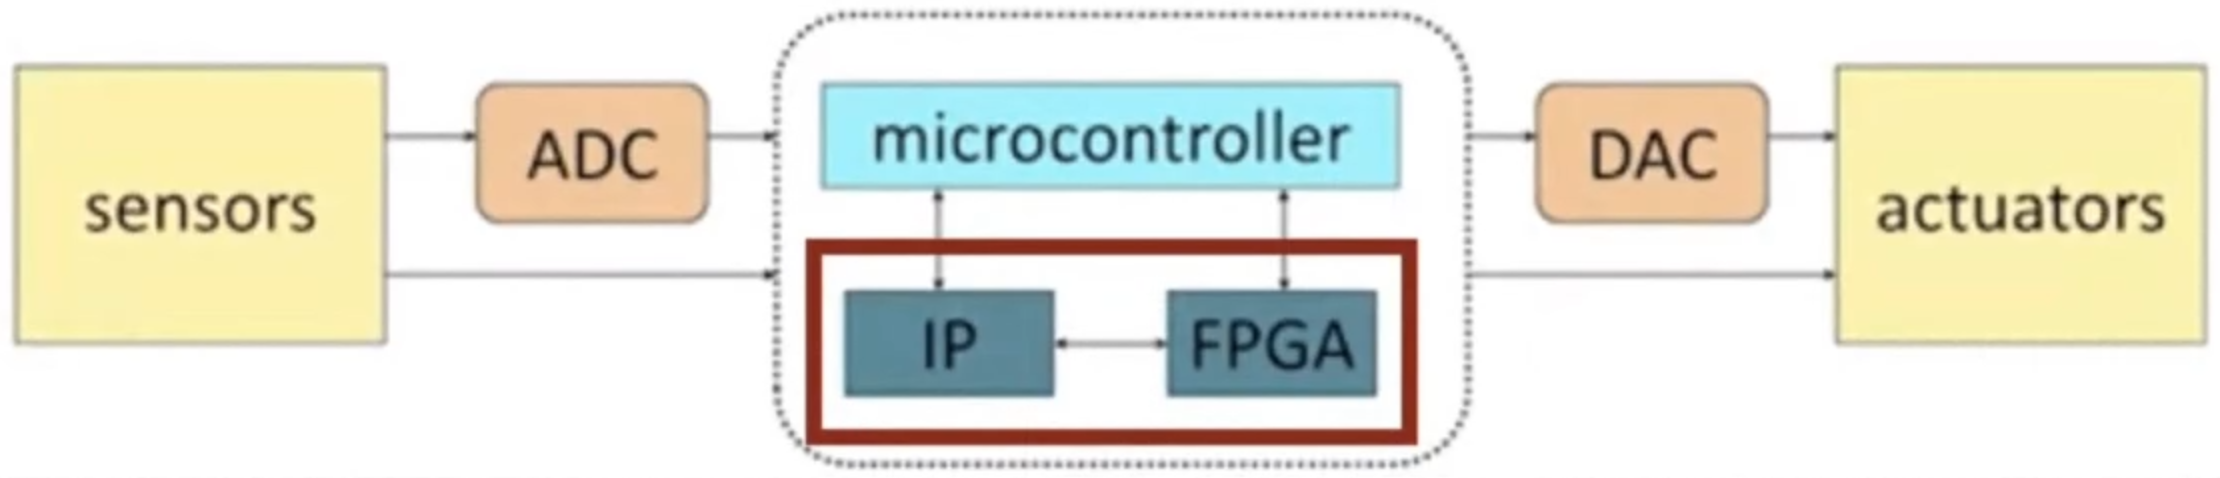
\includegraphics[scale=.35]{2021-03-19 16_58_28-DSO Elementos Sistema embebido.mkv.png}}
\end{figure}

\begin{description}
	\item[Microcontrolador] Es el componente que ejecuta un programa en un sistema integrado, y se encuentra en la zona central, se encarga de realizar el procesamiento.

	      Conectado a otros componentes del hardware, envía órdenes a los actuadores y recibe datos de los sensores.

	      Consta de CPU, RAM, ROM, puertos E/S y temporizadores.

	      Más lento que un microprocesador, menos memoria y menos funciones.

	      Requiere ser programado, se debe escribir el código del programa que va a realizar. El código se escribe en el host, un ordenador de sobremesa o laptop, y después se transfiere el programa del host al microcontrolador.
	\item[Cajas negras] Realizan parte del trabajo del microprocesador para reducir la carga, algunas tareas específicas. Algunos ejemplos son:
	      \begin{description}
		      \item[IP Core] Circuito integrado que desempeña una función que interactúa con el microcontrolador, y son baratos en un volumen alto. Muy útiles para tareas comunes como controlador de network (Ethernet, CAN)  o de audio/video (Audio Códec, Controlador VGA). Necesita interactuar con el microprocesador y se siguen unos protocolos de comunicación.

		      \item[FPGA - Field Programmable Gate Array] Matriz de puertas lógicas programable en campo, es un chip con una red de puertas de memoria RAM que se pueden configurar (establecer las conexiones entre chips o puertas), para realizar una serie de tareas, como puede ser filtrar una señal o comprimir video. Es más rápido que software, pero más lento que ASIC.

		      \item[DSP] Procesadores y compresores de señales digitales, tanto de audio como de video. Son más económicos que los procesadores, pero tiene capacidades más limitadas.

	      \end{description}
	\item[Conversores] Analógico-Digital sale de sensor, izquierda y el Digital-Analógico va al actuador, derecha. Los analógicos a digital son muy comunes, porque los sensores son analógicos y el microcontrolador es digital.
	\item[Sensores y actuadores] Toma medidas del medio que rodea al dispositivo y puede alterar el entorno. Sensores a la izquierda y actuadores a la derecha.
\end{description}

\section{Ejemplos de Sistemas embebidos que usamos}
\subsection{Arduino}

\begin{figure}[H]
	\ffigbox[\FBwidth]
	{\caption{Estructura Arduino}}
	{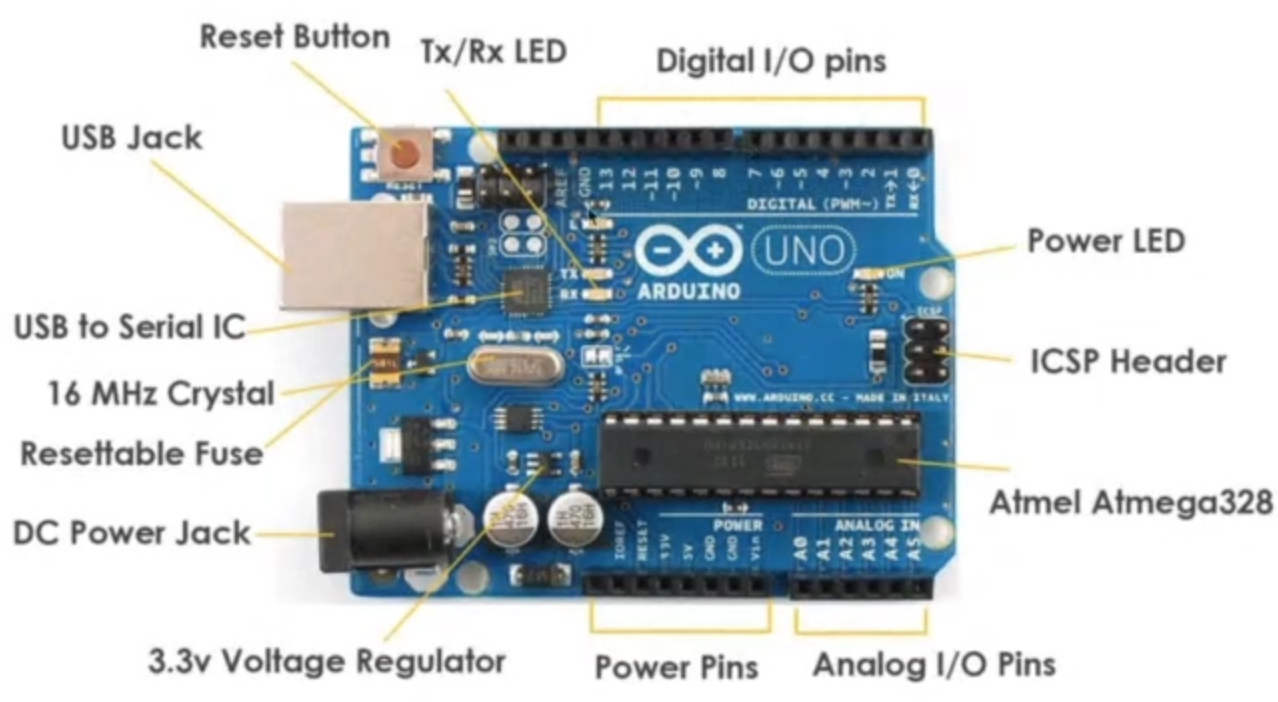
\includegraphics[scale=.5]{2021-03-19 17_31_12-DSO Elementos Sistema embebido.mkv.png}}
\end{figure}


Es una plataforma de código abierto sed para construir proyecto de electrónica.	Consta de una placa de circuito programable física (microcontrolador) y una pieza de software, o IDE (entorno de desarrollo) que se ejecuta en una computadora portátil o computadora personal utilizada para escribir y cargar código de computadora en la física. Tiene pines analógicos y digitales.

No necesita una pieza software separada para cargar un nuevo código en la placa.

Utiliza una versión simplificada de C++, lo que lo hace más fácil de aprender.

\textbf{Razones por la que se usa:} Es de código abierto, económico, multiplataforma, prototipos rápidos, entorno programable más simple y claro. Algunas también cuentan con conexión a Internet incorporada o la posibilidad de conectividad externa.

\textbf{Razones para no utilizarlos:} Poca memoria para datos y RAM, procesamiento, arquitectura basada en 8 bits, caro cuando se necesita a gran escala, mala calidad/precio, las empresas no les gusta que sea open source, no está aliado con proveedores y no da garantías.

\subsection{Raspberry Pi}

\begin{figure}[H]
	\ffigbox[\FBwidth]
	{\caption{Estructura Raspberry Pi}}
	{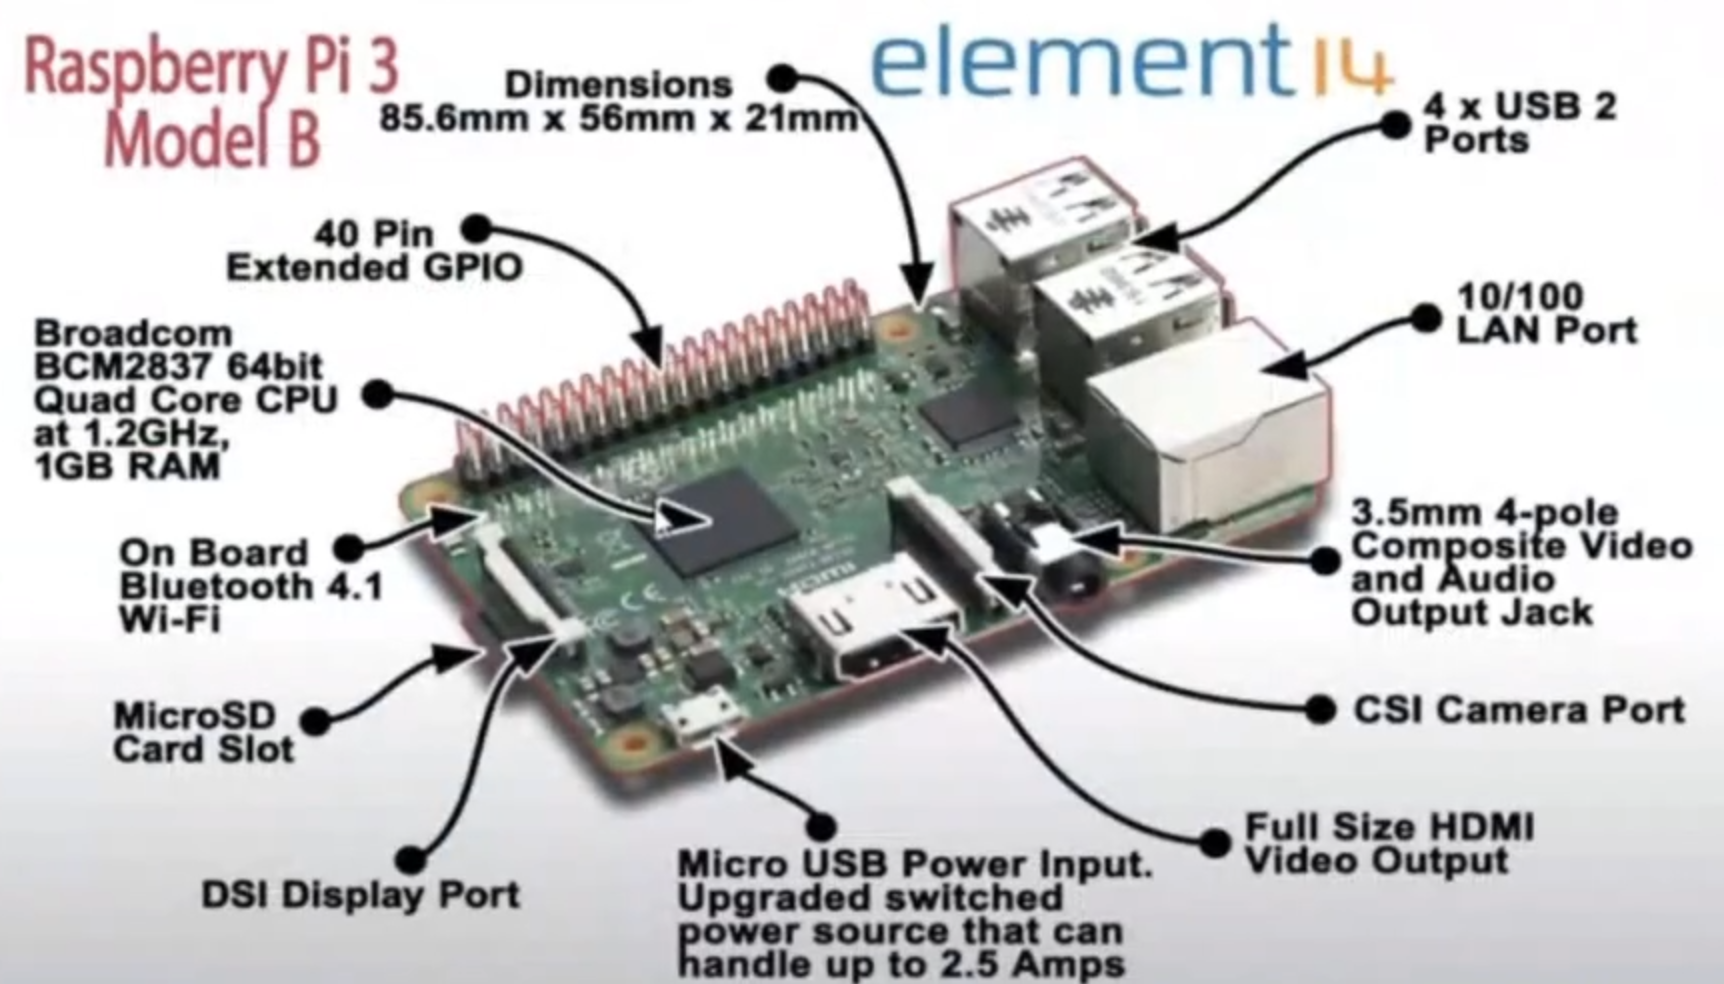
\includegraphics[scale=.4]{2021-03-19 17_48_46-DSO Elementos Sistema embebido.mkv.png}}
\end{figure}

Es una computadora de bajo costo del tamaño de una tarjeta de crédito que se conecta a un monitor de computadora o televisor y utiliza un teclado y un mouse estándar.

La Raspberry PI tiene una conexión GPIO de 40 pines, lo que facilita la conexión con el mundo exterior.


\begin{description}
	\item[GPIO] Significa entrada/salida de uso general. Estos pines son una interfaz física entre Raspberry Pi y el mundo exterior.

	      El Pi puede recibir información de sensores y actuadores, y controlar actuadores como LED, ejecutar motores y muchas otras cosas.

	      Hay 40 pines y proporcionan varias funciones diferentes.
	      \begin{itemize}
		      \item Los pines 27 y 28, ID SD e ID SC, son para conectar una EEPROM.
		      \item Pines 8 y 10, GPIO 14 y 15, son para comunicación UART puerto serie que transmite poca información (baja frecuencia), como USB, RFID, Bluetooth, GPS, GSM o GPRDS.
		      \item GPIO 2 y 3 (clock) se usan para I2C, comunicación entre placas, como un LCD, otras placas base (Raspberry, Arduino, ...) o un reloj de tiempo real.
		      \item GPIO 7, 8, 9, 10 y 11 implementan otro mecanismo de comunicación el SPI, que es la evolución del protocolo I2C, su función es comunicar full duplex, como SSD card, IP Core o Memoria Flash.
	      \end{itemize}

\end{description}
\textbf{Del cuestionario:}

\begin{itemize}
	\item Cuál de los siguientes NO es un beneficio de usar un sistema operativo?

	      La frecuencia del reloj del microprocesador se puede aumentar significativamente.
\end{itemize}

\subsection{Raspberry Pi vs. Arduino}
\begin{itemize}
	\item Raspberry usa un procesador de propósito general y Arduino un microprocesador.
	\item Raspberry Pi es más rápido (1.4 GHz vs. 16 MHz).
	\item Raspberry Pi puede administrar un espacio de direcciones más grande (procesador de 64 bits, frente a 8 bits).
	\item Raspberry Pi tiene más memoria: Arduino tiene 32 K Flash, 2 K RAM, 1 K EPROM; y Raspberry Pi SRAM de 1 GB, Micro SD.
	\item Raspberry Pi tiene niveles de voltaje de E/S más bajos (3.3 V frente a 5 V)
\end{itemize}

\begin{figure}[H]
	\ffigbox[\FBwidth]
	{\caption{Raspberry Pi vs. Arduino}}
	{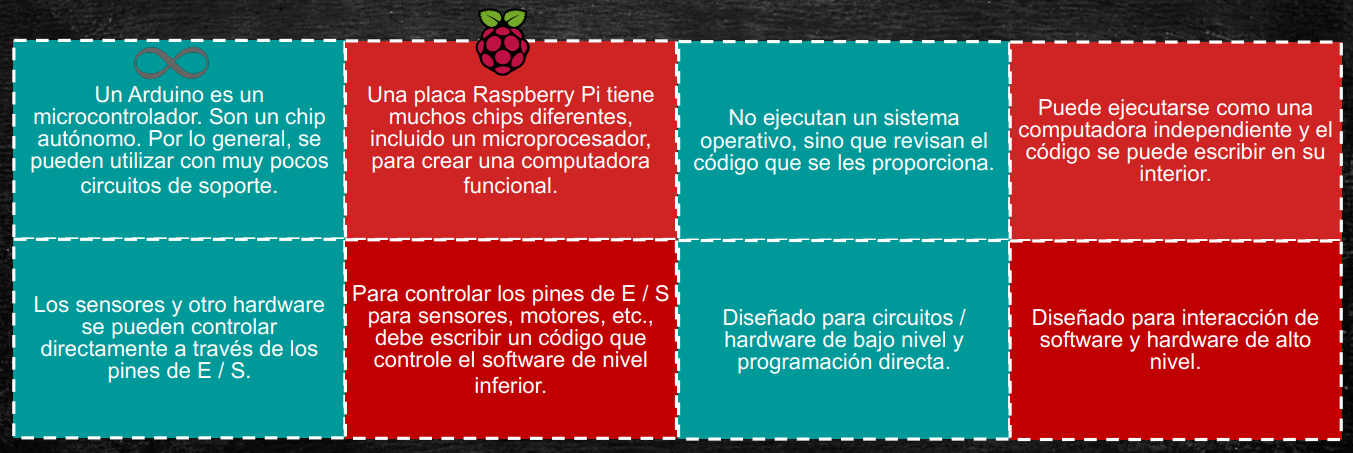
\includegraphics[scale=.62]{2021-03-24 19_03_44-Tema 03 - Gateways IoT - Sistemas Embebidos.png}}
\end{figure}
\pagebreak
\subsection{¿Es Raspberry Pi un dispositivo de IoT?}

\textbf{Similitudes:}
\begin{itemize}
	\item Conectividad de red e inteligencia computacional.
	\item Pequeño y barato (en relación con una PC).
	\item Puede interactuar directamente con sensores/actuadores a través de pines.
\end{itemize}


\textbf{Diferencias:}
\begin{itemize}
	\item La interfaz puede ser exactamente la misma que la de una PC con Linux: Las complejidades del sistema pueden ser visibles.
\end{itemize}

\section{Sistemas Operativos embebidos}
Es una parte opcional de la pila de software de un dispositivo, lo que significa que no todos los sistemas integrados tienen uno.

Proporciona una capa de abstracción para el software sobre el sistema operativo.
Administra los diversos recursos de hardware y software del sistema para garantizar que todo el sistema funciona de manera eficiente y confiable.

En nuestro caso tiene como función proporcionar una interfaz común (no tiene por qué ser gráfica) y abstracta a todos los elementos de hardware y que sea capaz de que las aplicaciones que se van a desarrollar sobre él se programen de la manera más fácilmente posible.

El núcleo del sistema operativo es el kernel, pero depende el SO embebido tendremos distintos tipos, algunos más robustos que tienen incluso interfaz gráfica o más ligeros que tienen la gestión de procesos y memoria.

\begin{figure}[H]
	\ffigbox[\FBwidth]
	{\caption{Capas Sistema Operativo}}
	{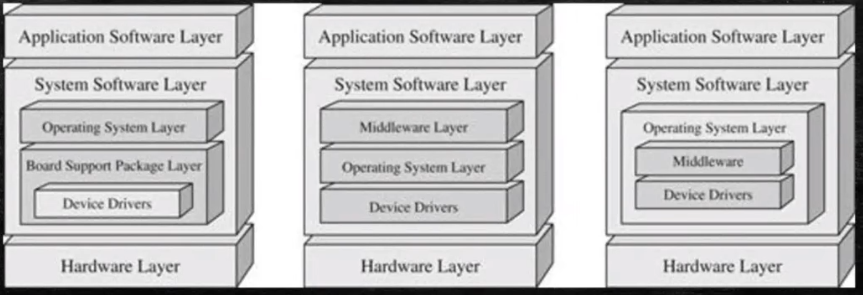
\includegraphics[scale=.6]{2021-03-25 09_19_18-2021-03-24 16-59-20.mkv.png}}
\end{figure}

\subsection{Principales Sistemas Operativos embebidos actuales}
Zephyr, Micrium, RTOS (Real Time Operative Systems), R IOT, VxWorks, ThreadX, MircroEJ, TinyOS, APACHE, ARMmbed, Contiki, Nucleus, Windows IoT, snappy, android things, Mongoose o mynewt.

\subsection{Requisitos de un Sistema Operativo Embebido}
\textbf{Restricciones de Hardware Heterogéneos}
\begin{itemize}
	\item Requisitos de CPU: Las operaciones no deben ser de carga alta, hay baja frecuencia.
	\item Requisito de Memoria: Suelen tener poca memoria (Arduino 4K).
	\item Características limitadas
	\item Soporte a Plataformas
\end{itemize}

\textbf{Autonomía}
\begin{itemize}
	\item Eficiencia energética: Como suspenderse bajo inactividad o protocolos de comunicación de bajo consumo.
	\item Stack de Red Adaptativo
	\item Fiabilidad, cuanto más tiempo pase antes de que necesite asistencia o ser remplazado, más autonomía.
\end{itemize}

\textbf{Programabilidad:}
\begin{itemize}
	\item API estándar: Gestionar procesos, servicios, tareas, threads, interrupciones, shockets...
	\item Lenguajes de Programación estándar, que nos permita utilizar la API para desarrollar aplicaciones.
\end{itemize}

\subsection{Capa de Software del Sistema}
\begin{figure}[H]
	\ffigbox[\FBwidth]
	{\caption{Modelo General SO embebido}}
	{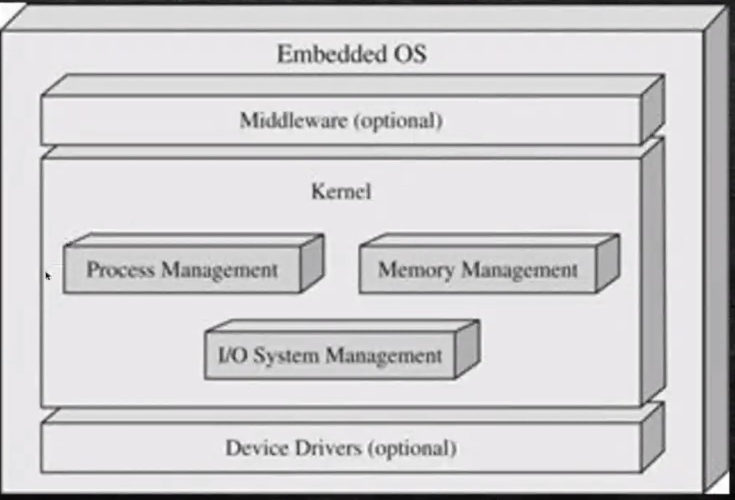
\includegraphics[scale=.5]{2021-03-25 10_06_39-2021-03-24 16-59-20.mkv.png}}
\end{figure}

Es un conjunto de librerías que proporcionan 3 grandes áreas de procesamiento: Gestión de tareas, de memoria y de Entrada/Salida. Dependiendo del SO puede incluir los drivers de los distintos dispositivos hardware que conectamos, o servicios de programación más refinados para tareas más complejas en el Middleware.

\subsubsection{Controladores de Dispositivos - Device Drivers}
Son las bibliotecas de software que sirven para interactuar con los distintos elementos hardware. Inicializan el hardware y administran el acceso al mismo mediante capas superiores de software. Por ejemplos los de GPIO de Raspberry Pi.

Todos los controladores de dispositivos generalmente se componen de todas o una combinación de las siguientes funciones: Inicio, Apagado, Lectura, Escritura, Deshabilitar o Habilitar hardware.

\textbf{Acciones:}
\begin{itemize}
	\item \textbf{Hardware Startup:} Inicialización del hardware tras el encendido o el restablecimiento.
	\item \textbf{Hardware Shutdown:} Configurando el hardware en su estado PowerOFF.
	\item \textbf{Hardware Disable:} Permitir que otro software desactive el hardware sobre la marcha.
	\item \textbf{Hardware Enable:} Permitir que otro software active el hardware sobre la marcha.
	\item \textbf{Hardware Acquire:} Permitir que otro software obtenga acceso singular (bloqueo) al hardware.
	\item \textbf{Hardware Release:} Permitir que otro software libere (desbloquee) hardware.
	\item \textbf{Hardware Read:} Permitir que otro software lea datos en el hardware.
	\item \textbf{Hardware Write:} Permitir que otro software escriba datos en el hardware.
	\item \textbf{Hardware Install:} Permitir que otro software instale nuevo hardware sobre la marcha.
	\item \textbf{Hardware Uninstall:} Permitir que otro software quite hardware instalado sobre la marcha.
	\item \textbf{Hardware Mapping:} Permite el mapeo de direcciones hacia y desde dispositivos de almacenamiento de hardware para leer y escribir datos.
	\item \textbf{Hardware Unmapping:} Permitiendo eliminar bloques de datos de dispositivos de almacenamiento de hardware.
\end{itemize}

\subsubsection{Kernel}

\begin{description}
	\item[Gestión de Procesos - Process Management] Como el sistema operativo administra y ve otro software en el sistema embebido.

	      \begin{description}
		      \item[Threads] Crear hilos, lanzarlos, controlarlos, terminarlos o sincronizarlos. Estos nos permiten tener varias tareas en ejecución de manera concurrente.
		      \item[Semaphores] Primitiva de sincronización, para evitar las condiciones de carrera.
		      \item[Priority scheduling] Determinar el orden en el que los hilos entran a ejecutar.
		      \item[Real-time signal extension] Interrupciones y señales, para activar notificaciones de aplicaciones asíncronamente.
		      \item[Timers] Mecanismo de notificación que nos avisa cuando se ha alcanzado o superado un determinado tiempo.
		      \item[IPC] Comunicación Inter-Proceso.
	      \end{description}

	      \paragraph{Gestión de multitareas y de procesos en sistemas embebidos}

	      Una de las principales diferencias de los SO embebidos es que no tenemos múltiples núcleos, donde en cada núcleo se podría ejecutar distintas cosas, lo que tenemos es un único núcleo que ejecuta una única tarea a la vez y va asignando rodajas a los procesos para dar la sensación de que se ejecutan varias en paralelo.

	      Como no se pueden hacer múltiples tareas a la vez, por lo que debemos tener un mecanismo que administre y planifique el orden de ejecución de los distintos procesos. Indicar cuando entran y salen, y el paso de datos.

	      La Raspberry Pi como tiene 4 núcleos se considera nano ordenador, no sistema embebido.


	      \paragraph{Implementación de procesos en Sistemas Operativos embebidos}

	      Las tareas están estructuradas como una jerarquía de tareas principales y secundarias, y cuando se inicia el kernel embebido, solo existe una tarea de la que se lanzan todas las demás.


	      \paragraph{Creación de tareas}
	      La creación de tareas en sistemas operativos integrados se basa principalmente en dos modelos, fork/exec (deriva del IEEE/ISO POSIX) y spawn (deriva de fork/exec).

	      \begin{itemize}
		      \item \textbf{fork:} Crea una copia del espacio de memoria de la tarea principal en lo que se asigna para la tarea secundaria, lo que permite que la tarea secundaria herede varias propiedades, como el código del programa y las variables, de la tarea principal.
		      \item \textbf{exec:} Se utiliza para eliminar explícitamente del espacio de memoria de la tarea secundaria cualquier referencia al programa principal y establece el nuevo código de programa que pertenece a la tarea secundaria para que se ejecute.
		      \item \textbf{spawn model:} Crea un espacio de direcciones completamente nuevo para la tarea secundaria. La llamada al "modelo de generación" permite definir el nuevo programa y los argumentos para la tarea secundaria.
	      \end{itemize}

	      \textbf{Spawn model:} No tiene espacios duplicados, optimiza el espacio de memoria, no gasta tanta memoria como fork/exec. Es más complicado compartir propiedades entre procesos.

	      \textbf{fork/exec:} Nos permite coordinar de una manera más sencilla y compartir propiedades, pero es más lenta y requiere más memoria (que es limitada) porque tiene que copiar y eliminar.

	      \paragraph{Planificador de Tareas - Scheduler:} Es el que nos dice cuándo y cuanto tiene va a ejecutar cada una de las tareas, va metiendo y sacando de la CPU. El programador clasifica las tareas en READY, RUNNING y BLOCK.

	      \paragraph{Factores clave del Scheduling}
	      Lo critico es la efectividad y la eficiencia en cuanto al tiempo de respuesta en cambiar entre tareas y elegir cuál es la va a continuación.
	      \begin{itemize}
		      \item \textbf{Tiempo de respuesta - Response Time:} Tiempo para que el programador haga que el contexto cambie a una tarea lista e incluye el tiempo de espera de la tarea en cola lista.
		      \item \textbf{Turnaround time:} El tiempo que tarda un proceso en completarse.
		      \item \textbf{Overhead:} El tiempo y los datos necesarios para determinar que tareas se ejecutan a continuación.
		      \item \textbf{Fairness:} Ser capaz de realizar una partición equitativa entre todas las tareas que están pendientes de ejecución. ¿Cuáles son los factores determinantes en cuanto a qué procesos llegan a ejecutarse?
		      \item \textbf{Throughput:} Procesar tantas tareas como sea posible en un periodo de tiempo determinado. tareas por unidad de tiempo.
		      \item \textbf{Starvation:} Donde una tarea nunca llega a ejecutarse, nunca recibe una rodaja de tiempo.
	      \end{itemize}


	      \paragraph{Preventivo vs. No preventivo}

	      Utilizar el término más parecido a la terminología inglesa, Expropiativo y No expropiativo.

	      \begin{itemize}
		      \item \textbf{Non-pre-emptive - No expropiativo - Apropiativo:} No se le puede expulsar. Las tareas reciben el control de la CPU maestra hasta que finalizan su ejecución, independientemente del tiempo o la importancia de las otras tareas que están en espera.

		            Ejemplos: FCFS, SPF o SJF, Prioridades

		      \item \textbf{Pre-emptive - Expropiativo - No apropiativo:} Se les puede expulsar de las CPU cuando acaba su rodaja, se dividen los procesos en rodajas de duración fija. El SO fuerza el cambio de contexto en una tarea, ya sea que una tarea en ejecución haya terminado de ejecutarse o este cooperando con el cambio de contexto.

		            Ejemplos: Round Robin, SRTF, Colas Multinivel
	      \end{itemize}

	      \paragraph{Planificación e Raspberry Pi OS}
	      \begin{itemize}
		      \item Opera en todos los componentes.
		      \item Solo se ejecuta una tarea a la vez.
		      \item El planificador es un componente independiente.
		      \item El programador predeterminado es una cola FIFO simple.
		      \item La planificación es consciente de la energía, y pone el procesador en suspensión cuando no hay ninguna tarea en la cola.
	      \end{itemize}

	      \paragraph{Manejo de señales e interrupciones} Cuando llega una interrupción externa, saca el proceso de la CPU y atiende la interrupción ejecutando la rutina correspondiente, y vuelve al proceso previo.

	      \paragraph{Sincronización y comunicación entre tareas} Nos permite que las distintas subtareas compartan datos, la manera más sencilla es utilizando espacios de memoria compartidos.

	\item[Memory Management] El espacio del sistema embebido es compartido por todos los diferentes procesos, por lo que es necesario administrar el acceso y la asignación de partes del espacio de memoria. Los procesos de memoria para tener en cuenta:
	      \begin{description}
		      \item[Process memory locking] Ser capaz de bloquear y evitar los accesos indebidos al espacio de memoria de otros procesos.
		      \item[Memory mapped files] Llevar a memorias secundarias algunos mapas o páginas que tenga en función de las restricciones.
		      \item[Shared memory object] Implementar variables, objetos o espacios de memoria compartidos en distintos procesos para favorecer su sincronización.
	      \end{description}

	      \paragraph{Modo de usuario vs. Modo kernel}
	      La forma en que los sistemas operativos administran el espacio de memoria lógica difiere de un sistema operativo a otro, pero los núcleos generalmente ejecutan el código del núcleo en un espacio de memoria separado de los procesos que ejecutan código de nivel superior (es decir, middleware y código de capa de aplicación).


	\item[I/O System Management] Se encarga de cómo vamos a almacenar o permitir que los procesos entre sí accedan al espacio de almacenamiento secundario. Lo que queremos es una interfaz estándar para que puedan acceder a todos los espacios de almacenamiento independientemente del hardware y driver que tenga implementado.

	      Los dispositivos de E/S también deben compartirse entre los diversos procesos y, por tanto, al igual que con la memoria, el acceso y la asignación de un dispositivo de E/S deben administrarse.

	      \begin{figure}[H]
		      \ffigbox[\FBwidth]
		      {\caption{Gestión de archivos en Sistemas Embebidos}}
		      {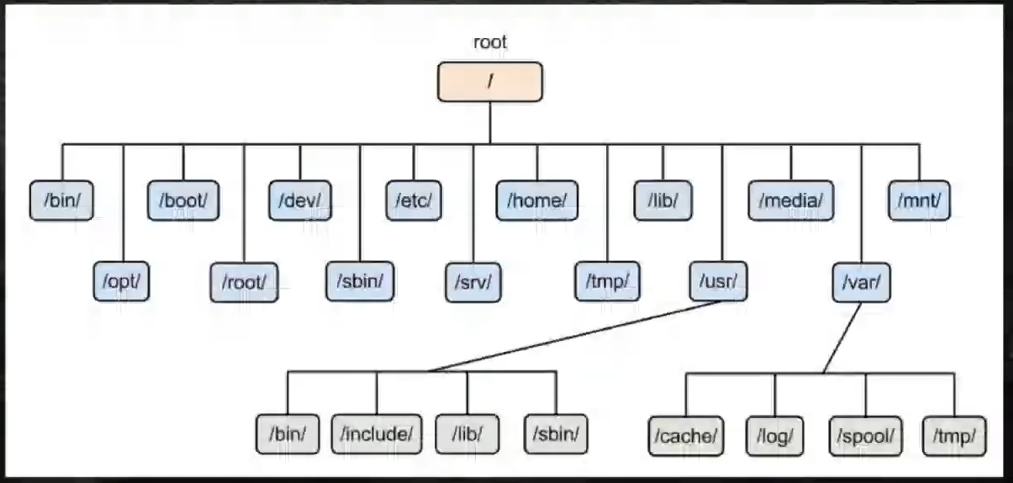
\includegraphics[scale=.5]{2021-03-25 11_52_40-2021-03-24 16-59-20.mkv.png}}
	      \end{figure}

\end{description}

\subsubsection{Middleware}

Cualquier software del sistema que no es kernel del sistema operativo, controladores de dispositivos o las aplicaciones que se van a desarrollar. Se puede encontrar dentro de los controladores de los dispositivos, del software del SO o independiente sobre estos dos.

\textbf{Razones para usar Middleware}
\begin{itemize}
	\item \textbf{Adaptabilidad - Adaptability:} Permite que el middleware superpuesto y/o aplicaciones integradas se adapten a los cambios en la disponibilidad de los recursos.
	\item \textbf{Conectividad - Connectivity:} Proporciona al middleware superpuesto y/o aplicaciones integradas la capacidad de comunicarse de forma transparente entre aplicaciones de distintos dispositivos, a través una interfaz estándar y amigable.
	\item \textbf{Flexibilidad y Escalabilidad - Flexibility and Scalability:} Permite que el middleware y/o aplicaciones integradas sean configurables y personalizables en términos de funcionalidad según los requisitos de la aplicación.
	\item \textbf{Portabilidad - Portability:} Permite que las aplicaciones integradas y/o middleware superpuestas se ejecuten en diferentes sistemas integrados con diferentes capas de software y/o hardware.
	\item \textbf{Seguridad - Security:} Garantiza que el middleware superpuesto y/o las aplicaciones integradas tengan acceso autorizado a los recursos del sistema.
\end{itemize}

\textbf{Tipos de Middleware}
\begin{itemize}
	\item \textbf{Middleware básico - core:} Tiene un propósito más general y es el más común. Sirve como base para el más complejo y está relacionado con la gestión de sistemas de archivos, las comunicaciones (Controladores de Red) y elementos que permitan virtualizar el funcionamiento.
	\item \textbf{Middleware complejo:} Middleware especifico del mercado, mensajería y comunicaciones complejas, mensajería distribuida y orientada a mensajes, y transacciones distribuidas.
\end{itemize}

Aun así, puede ser middleware \textbf{propietario}, que significa que es un software cerrado respaldado por una empresa que lo licencia a otra para su uso, o puede ser \textbf{abierto}, lo que significa que puede ser implementado y/o licenciado por cualquier parte interesada.

\subsection{Capa de Software de Aplicación}
Se encuentra en la parte superior de la capa de software del sistema y depende del software del sistema, o administra y lo ejecuta.

Es el software dentro de la capa de aplicación el que define inherentemente que tipo de dispositivo es un sistema integrado, porque la funcionalidad de una aplicación representa al más alto nivel el propósito de ese sistema integrado y realiza la mayor parte de la interacción con los usuarios o administradores de ese dispositivo.

Se pueden dividir en aplicaciones integradas \textbf{específicas del mercado} (implementada en un solo tipo de dispositivo) o de \textbf{propósito general} (se pueden implementar en varios tipos de dispositivos).
\pagebreak
\section{Preguntas Test 2}
\begin{enumerate}
	\item Seleccione la frase incorrecta con respecto a la definición de sistemas embebidos:

	      d. PDA o web pads son ejemplos típicos de sistemas embebidos.

	\item ¿Por qué POSIX es muy relevante en el área de sistemas operativos integrados?

	      b. Porque proporciona una interfaz de programación estándar para sistemas operativos embebidos.

	\item Seleccione la afirmación correcta con respecto a las señales/interrupciones del sistema operativo integrado:

	      b. Las interrupciones son indicadores de que un evento asincrónico ha sido generado por algún evento externo.

	\item Seleccione la afirmación correcta con respecto a la interfaz GPIO de Raspberry Pi:

	      a. Los pines UART se pueden usar para comunicar su Raspberry Pi con otros dispositivos que tengan una interfaz serie.

	\item Las placas de desarrollo de microcontroladores...

	      a. incluyen hardware para programar microcontroladores.

	\item Seleccione la afirmación correcta con respecto a las funcionalidades de los controladores del sistema operativo integrado:

	      b. La funcionalidad de instalación de hardware permite que otro software instale nuevo hardware sobre la marcha.

	\item Seleccionar la afirmación incorrecta:

	      d. Raspberry Pi está diseñado para la integración de hardware de bajo nivel.

	\item Las responsabilidades de gestión de la memoria en el sistema operativo embebido incluye:

	      a. Determinar qué procesos cargar en el espacio de memoria disponible.

	\item Seleccionar la afirmación incorrecta:

	      ?? a. Windows IoT no es un sistema operativo embebido IoT.

	      c. Debian no es un sistema operativo embebido IoT.

	\item La placa Arduino One no incluye

	      a. Una ranura para tarjeta Micro SD.
\end{enumerate}


\chapter{Tema 5: Protocolos para gestionar dispositivos IoT en la nube}

\section{Edge Interface, Message Broker y Message Bus}

Se encargan de enrutar y recibir los mensajes de datos que proporcionan los dispositivos IoT, tratan con la transmisión de mensajes con el mundo físico, especialmente dispositivos y sensores heterogéneos. Se trata de encapsular de una manera estandarizada los métodos, tecnologías o protocolos de transporte que utilizan los dispositivos IoT para conectarse a internet.

Los protocolos estándar son las herramientas que unen y encapsulan datos sin procesar de un sensor a algo significativo y formateado para que la nube lo acepte.

Los protocolos dominantes son MQTT y CoAP.

\begin{figure}[H]
	\ffigbox[\FBwidth]
	{\caption{Protocolos de comunicación}}
	{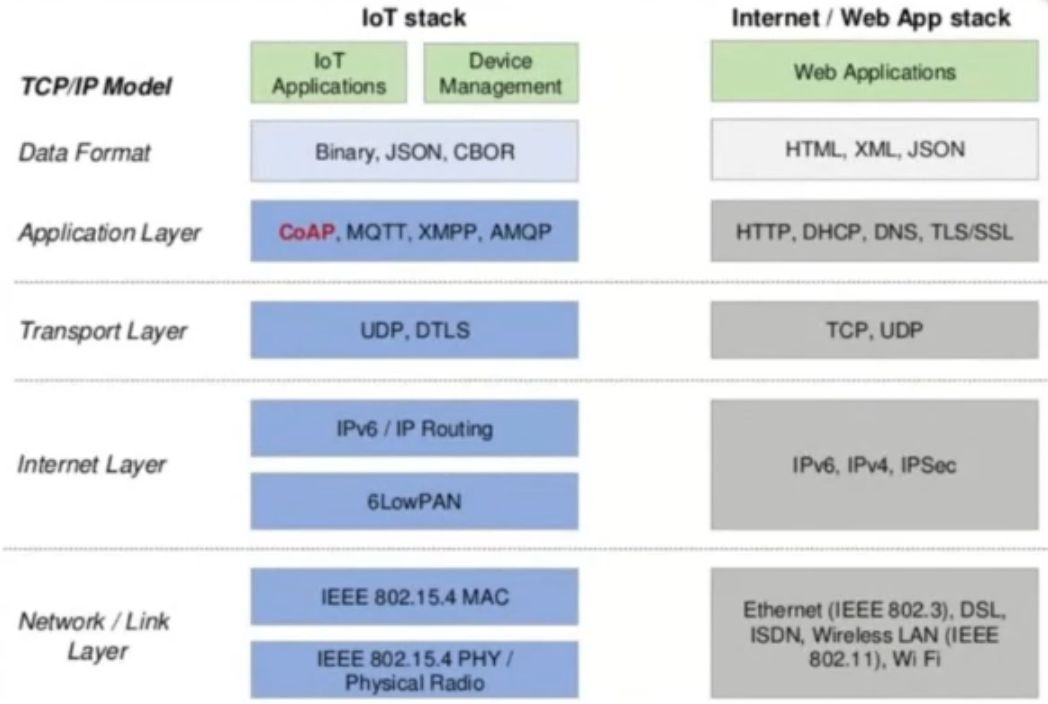
\includegraphics[scale=.5]{2021-04-08 09_06_45-2021-04-07 17-01-12.mkv.png}}
\end{figure}

El problema de usar TCP y HTTP (basado en TCP) es que son muy ricos en información que es una ventaja, pero en el caso de los dispositivos IoT se dispone de recursos limitados, por lo que se preferirá aquellos más ligeros.

\section{Middleware Orientado a Mensajes}

Se basan en una cola de mensajes; CORBA, MQTT, AMQP o XMPP son algunos de los protocolos que lo utilizan.

El servicio de mensajería consta de 3 partes; Publisher (publicador, emisor), Broker (gestor de mensajes, retransmisor) y Subscriber (suscriptor, receptor).
\begin{itemize}
	\item El publicador se conecta y entonces puede enviar datos por un canal (topic).
	\item El broker confirma las conexiones y hace de intermediario, recibiendo y retransmitiendo.
	\item El suscriptor se conecta y pide recibir los mensajes de un canal (topic), y el broker se los irá enviando.
\end{itemize}


\begin{figure}[H]
	\ffigbox[\FBwidth]
	{\caption{Comunicación orientada a mensajes}}
	{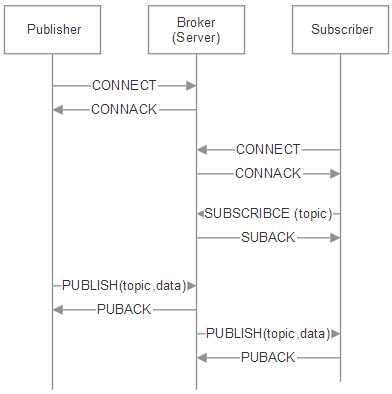
\includegraphics[scale=.5]{2021-04-08 09_17_44-2021-04-07 17-01-12.mkv.png}
		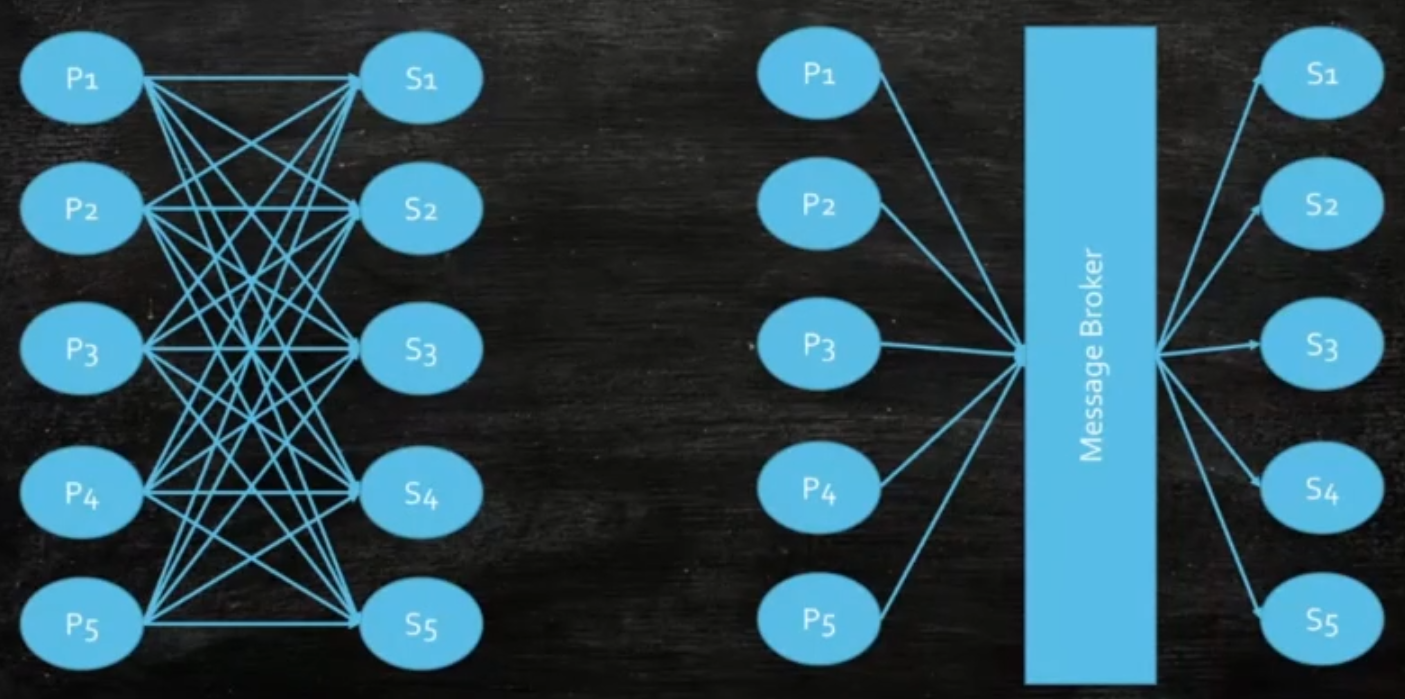
\includegraphics[scale=.22]{2021-04-08 09_20_09-2021-04-07 17-01-12.mkv.png}}
\end{figure}

El broker hace como intermediario de los publicadores y suscriptores, de esta manera se reduce el acoplamiento y es más fácil escalar el sistema.

A diferencia de HTTP, no es necesario que el publicador sepa a quién enviárselo, de esta manera se reduce también el consumo de recursos. Al igual los suscriptores no tienen que consultar a un montón de publicadores, solo al broker.

\newpage

\section{Servicio RESTful}

Es la alternativa a los protocolos basados en mensajes. Es asíncrono el intercambio de mensajes. Por ejemplo: CoAP

En un modelo RESTful el servidor posee el estado de un recurso, sabe en qué estado se encuentra.
La recepción de peticiones y la recepción de respuesta es independiente del estado. Se suele utilizar cuando quiero enviar datos a un servidor o los quiero recuperar.

Envía con post y recibe con get, resolviendo el URL.

Utiliza directamente el protocolo HTTP, todos están sobre este, mediante una URL podemos identificar el path.
Al emplear HTTP son protocolos muy exigentes en el ámbito de comunicaciones, requiere mayor cabecera y número de intercambios de mensajes.

\begin{figure}[H]
	\ffigbox[\FBwidth]
	{\caption{Servicio RESTful}}
	{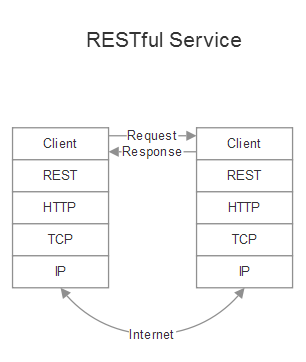
\includegraphics[scale=.7]{2021-04-08 09_36_12-2021-04-07 17-01-12.mkv.png}}
\end{figure}

\section{MQTT - Message Queuing Telemetry Transport}
Protocolo de cola de mensajes, es el protocolo de intercambio de mensajes en el ámbito IoT por excelencia.

Se empezó a trabajar en el en 1993 por IBM, para comunicar dispositivos en lugares remotos, con latencias altas y bajo ancho de banda.

Normalmente hay un suscriptor, un broker y un publicador, que funcionan como se ha descrito arriba (uno crea los topic, otro los gestiona y el último lo recibe).

Se debe tener en cuenta cuál es el tamaño máximo de los mensajes según el proveedor (IBM Watson allows for payload sizes up to 128 kB, while Google supports 256 kB), dado que admite cualquier archivo hay que cuidar de esto, aunque se recomienda que se envíen en formato JSON o en binario, porque son los mejores para conexiones inestables y poco almacenamiento.

\subsection{Desarrollo:}
\begin{itemize}
	\item 1993 - Se comienza a trabajar en él.
	\item 1999 - Andy Standford-Cark y Arlen Nipper fueron los autores de la primera versión del protocolo.
	\item 2010 - MQTT fue lanzado libre de regalías, royalties (se podía utilizar sin pagar).
	\item 2012 - Se lanzó la primera versión de Mosquitto.
	\item 2013 - MQTT-SN que fue especificado y diseñado para funcionar sobre UDP, Zigbee y otros transportes.
	\item 2014 - MQTT se convirtió en un estándar OASIS (de comunicaciones).
	\item 2018 - Se aprobó la versión MQTT v5 (aunque no es la más extendida).
\end{itemize}

\subsection{Objetivos:}
\begin{itemize}
	\item Debe ser fácil de implementar.
	\item Disponer de una calidad de servicio.
	\item Ser ligero y eficiente en ancho de banda, debe dar soporte a dispositivos con poco ancho de banda y consumo de energía.
	\item Ser agnóstico en cuanto al tipo de datos, puede tratar cualquier tipo de datos.
	\item Tener conciencia continua de la sesión.
	\item Abordar problemas de seguridad.
\end{itemize}

\subsection{Estructura de un paquete MQTT}
\begin{itemize}
	\item \textbf{Cabecera:} Indica que tipo de mensaje que estamos mandando y algunos flags.
	\item \textbf{Longitud del paquete}
	\item \textbf{Cabecera adicional (opcional)}: de longitud variable, de uso marginal.
	\item \textbf{Payload (datos):} Puede tener un tamaño variable, que por protocolo son 256 MB máximo, pero dependiendo del proveedor puede ser menor.
\end{itemize}

\begin{figure}[H]
	\ffigbox[\FBwidth]
	{\caption{Estructura de un paquete MQTT}}
	{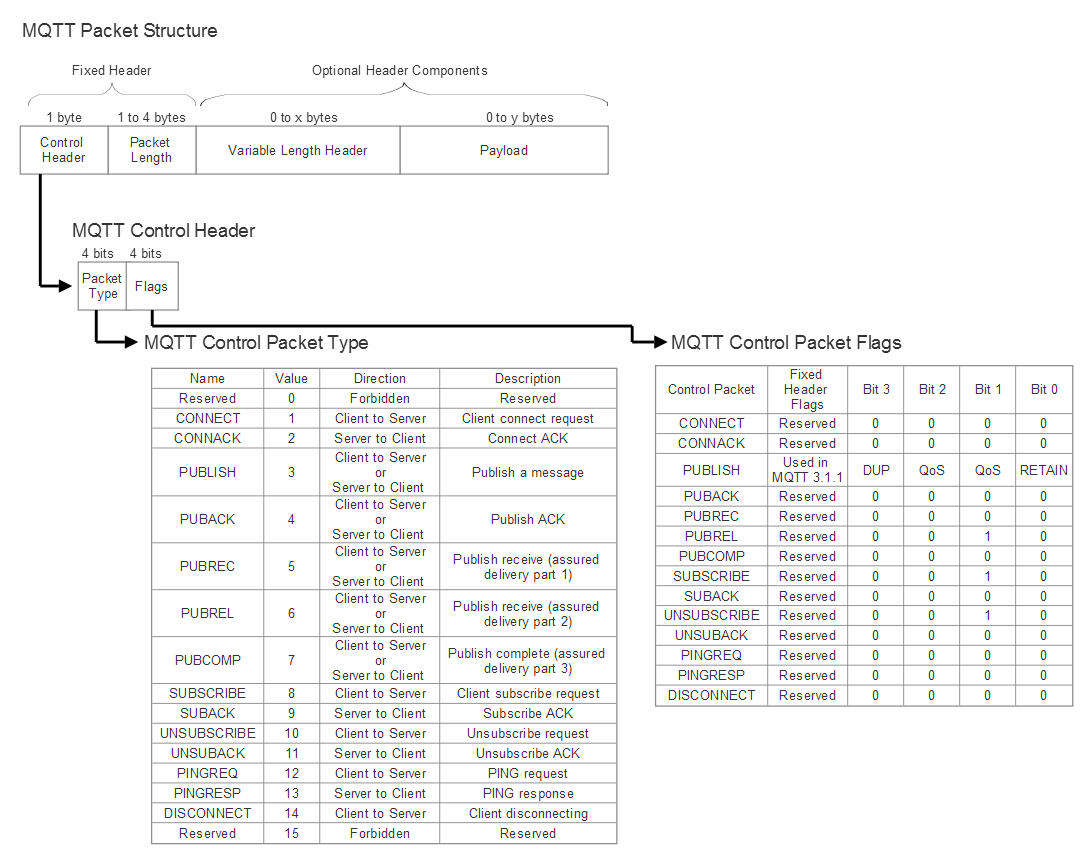
\includegraphics[scale=.5]{f4bd0f8a-2e92-4cdd-abfc-c7b067788d4a.png}}
\end{figure}

\subsection{Tipos de mensajes}
\subsubsection{CONNECT (cliente a servidor)}
Solicitud de conexión con el broker.

Solo es obligatorio el identificador de cliente (en nuestro caso lo administra paho), opcionalmente se puede proporcionar nombre de usuario, contraseña, keep alive o última voluntad.

\subsubsection{CONNECT (servidor a cliente)}
Es el ACK de la conexión recibida, responde al CONNECT con un código (RC).
\begin{description}
	\item[0] Conexión satisfactoria.
	\item[1] Conexión rechazada, versión de MQTT inaceptable.
	\item[2] Conexión rechazada, cliente identificado es UTF-8 y el servidor no lo permite.
	\item[3] Conexión rechazada, servidor no disponible.
	\item[4] Conexión rechazada, nombre o contraseña incorrecta.
	\item[5] Conexión rechazada, el cliente no tiene permiso de conexión.
\end{description}

\subsubsection{PUBLISH}
Publicar datos en una rama del canal.

Necesita un identificador de paquete/mensaje, nombre del canal (topic), nivel de calidad del servicio, retain y los datos (payload) son opcionales.

\subsubsection{SUBSCRIBE}
Suscribirse a un canal.

Requiere identificador de paquete, tópico al que se suscribe, nivel de calidad de servicio. Opcionalmente topic\_2 y qos2. Poniendo llaves en el topic, con el nombre dentro, se suscribe a todos. /uc3m/aulas/{aulas}/temperature

\subsection{Elementos de los mensajes}

\subsubsection{Last will - Ultima voluntad}
Es el mensaje que se envía a todos los suscriptores de un canal cuando se pierde la conexión de un publicador. Este parámetro se introduce al inicio.

\subsubsection{Retain}
En el indicamos si queremos que se retenga el mensaje hasta que sea confirmada la recepción por todos los suscriptores.

\subsubsection{Keep alive}
Indica cada cuanto tiempo se envía un mensaje al suscribirse, si no se recibe uno en 1,5 veces este valor se envía la última voluntad a los suscriptores. El servidor tiene un temporizador para controlar los tiempos.

\textbf{Desconexión inesperada de publicadores:} Se puede deber a quedarse sin batería, internet o no enviar el disconnect.
\begin{itemize}
	\item Conexión con petición de almacenamiento de "última voluntad"
	\item Almacenamiento de petición de "última voluntad"
	\item Confirmación de conexión.
	\item El publicador publica mensajes.
	\item El suscriptor recibe mensajes.
	\item El cliente inesperadamente deja de responder.
	\item El broker envía el mensaje de "última voluntad" a los suscriptores.
\end{itemize}
En caso de que el cliente no tenga nada que enviar envía periódicamente PINGRESP para que no piense que se ha muerto y se reinicie su temporizador.


\subsubsection{QoS - Calidad del servicio}
Son los aseguramientos de entrega de los mensajes enviados por un publicador. Nos permite indicar como queremos que sea la conexión respecto a la recepción de los mensajes.

\begin{description}
	\item[0 - Transmisión no asegurada] Es un proceso de entrega de mejor esfuerzo sin que el receptor reconozca un mensaje o el remitente vuelve a intentar transmitir. No se asegura de la entrega de todos los mensajes, si no llega se pierde.

	      Debe usarse cuando no se necesita la cola de mensajes, para conexiones por cable o sistemas muy limitado en ancho de banda.

	      \textbf{Orden de los eventos}
	      \begin{enumerate}
		      \item El dispositivo publicador se conecta al broker.
		      \item El suscriptor se conecta al broker.
		      \item El publicador publica un mensaje a través del broker.
		      \item El broker envía un mensaje al suscriptor con la información por el publicador.
	      \end{enumerate}

	      \begin{figure}[H]
		      \ffigbox[\FBwidth]
		      {\caption{QoS 0}}
		      {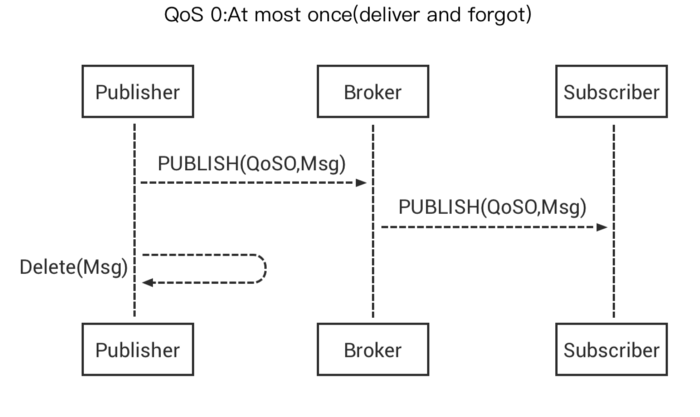
\includegraphics[scale=.5]{0_1NSybQWdhHvVhnTb.png}}
	      \end{figure}
	\item[1 - Transmisión asegurada] Asegura la entrega al menos una vez, puede recibirse el mismo mensaje varias veces. Produce más tráfico, el receptor envía un acuse de recibo con una respuesta PUBACK. Debería ser el uso predeterminado, más rápido que el 2 y reduce el costo de transmisión.

	      El publicador almacena el mensaje hasta que recibe la confirmación del broker de que se ha enviado al suscriptor. Se desentiende cuando sabe que se ha enviado.

	      El broker cunado recibe el mensaje lo almacena, envía al suscriptor, avisa del envío al publicador y hasta que no recibe la confirmación de los suscriptores no elimina el mensaje.

	      El suscriptor cuando recibe el mensaje confirma la recepción al broker.

	      \textbf{Orden de los eventos}
	      \begin{enumerate}
		      \item El dispositivo publicador A se conecta al broker.
		      \item El suscriptor B se conecta al broker.
		      \item El publicador publica un mensaje a través del broker.
		      \item El publicador A almacena el mensaje enviado.
		      \item El broker almacena el mensaje enviado por el publicador A.
		      \item El broker envía un mensaje al suscriptor B con la información enviada por el publicador A.
		      \item El broker notifica al publicador A que se ha enviado el mensaje.
		      \item El publicador A elimina el mensaje enviado.
		      \item El suscriptor B confirma que ha recibido el mensaje.
		      \item El broker elimina el último mensaje enviado por el publicador A.
	      \end{enumerate}

	      \begin{figure}[H]
		      \ffigbox[\FBwidth]
		      {\caption{QoS 1}}
		      {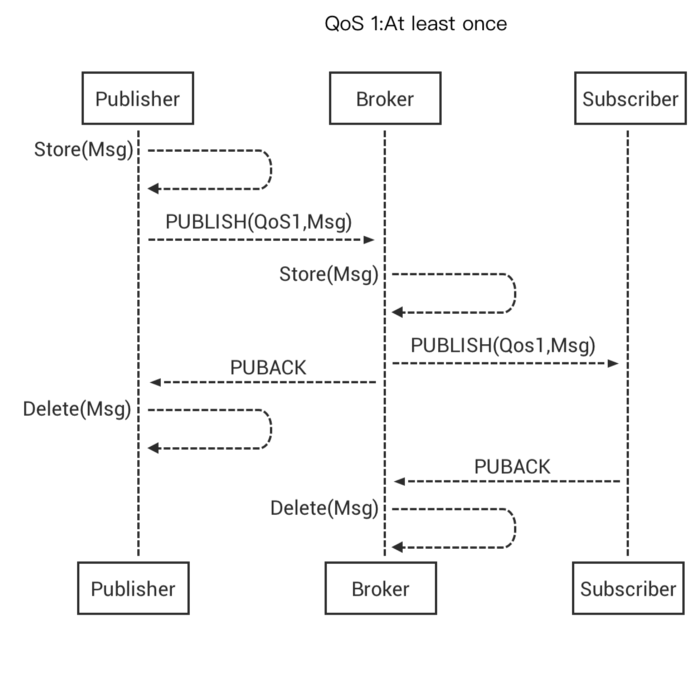
\includegraphics[scale=.35]{0_b4pvXUWp6MVnAAFy.png}}
	      \end{figure}
	\item[2 - Servicio asegurado en aplicaciones] Asegura la entrega, pero solo se recibirá el mensaje una única vez por suscriptor. Informa tanto al remitente como al receptor que se ha transmitido correctamente, se confirman todos los mensajes incluidas las confirmaciones de entregas.

	      Se usa para aplicaciones de misión crítica, sobre todo en aquellas circunstancias en las que recibir un mensaje duplicado podría provocar fallos.

	      \textbf{Orden de los eventos}
	      \begin{enumerate}
		      \item El dispositivo publicador A se conecta al broker.
		      \item El suscriptor B se conecta al broker.
		      \item El publicador A almacena el mensaje enviado.
		      \item El publicador A publica un mensaje a través del broker.
		      \item El broker almacena el mensaje enviado por el publicador A.
		      \item El broker envía un mensaje al suscriptor B con la información enviada por el publicador A.
		      \item El suscriptor B confirma que ha recibido el mensaje.
		      \item El broker envía al publicador A la confirmación de recepción de mensaje.
		      \item El publicador A envía la confirmación de la eliminación del mensaje al broker.
		      \item El broker informa al suscriptor B de la eliminación del mensaje.
		      \item El suscriptor B confirma al broker la recepción del aviso de eliminación del mensaje.
		      \item El suscriptor B elimina la información de estado de recepción del mensaje.
		      \item El broker confirma al publicador A la confirmación de la recepción del aviso de eliminación del mensaje por parte del suscriptor B.
		      \item El broker elimina el último mensaje enviado por el publicador A.
		      \item El publicador A elimina el mensaje enviado.
	      \end{enumerate}

	      Error en la imagen: el broker guardaría el mensaje después de recibirlo.
	      \begin{figure}[H]
		      \ffigbox[\FBwidth]
		      {\caption{QoS 2}}
		      {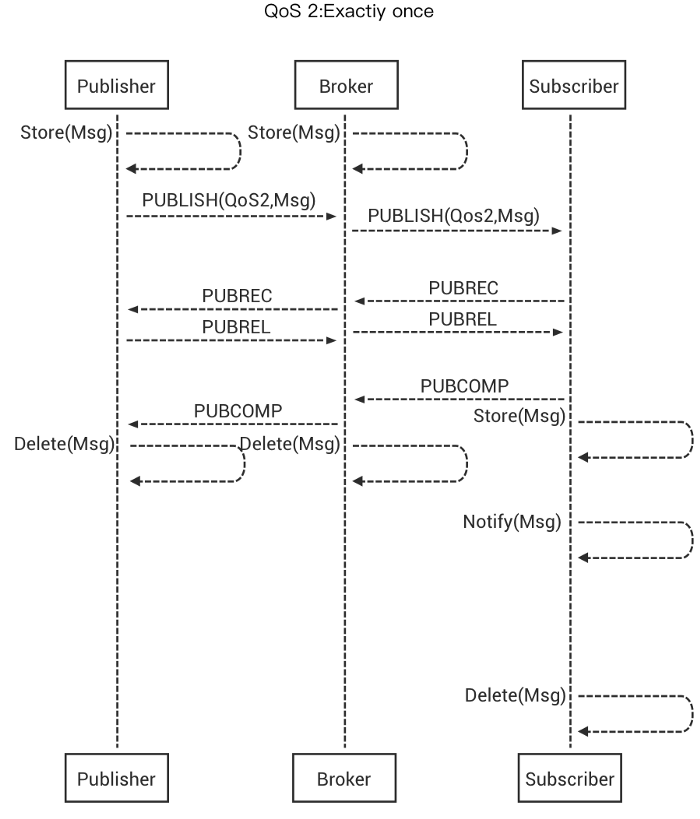
\includegraphics[scale=.2]{0_G6zwc_VftJ4AcueS.png}}
	      \end{figure}
\end{description}
\pagebreak
\section{MQTT-SN - Message Queuing Telemetry Transport for Sensor Networks}
Se utiliza en los casos en los que se quiere conectar sensores que se encuentran en lugares remotos, tienen problemas de batería, tiene una conexión inalámbrica débil o la conexión requiere mucha energía. En los que hay que optimizar los recursos.


\subsection{Elementos de estas redes:}
\begin{figure}[H]
	\ffigbox[\FBwidth]
	{\caption{Estructura MQTT-SN}}
	{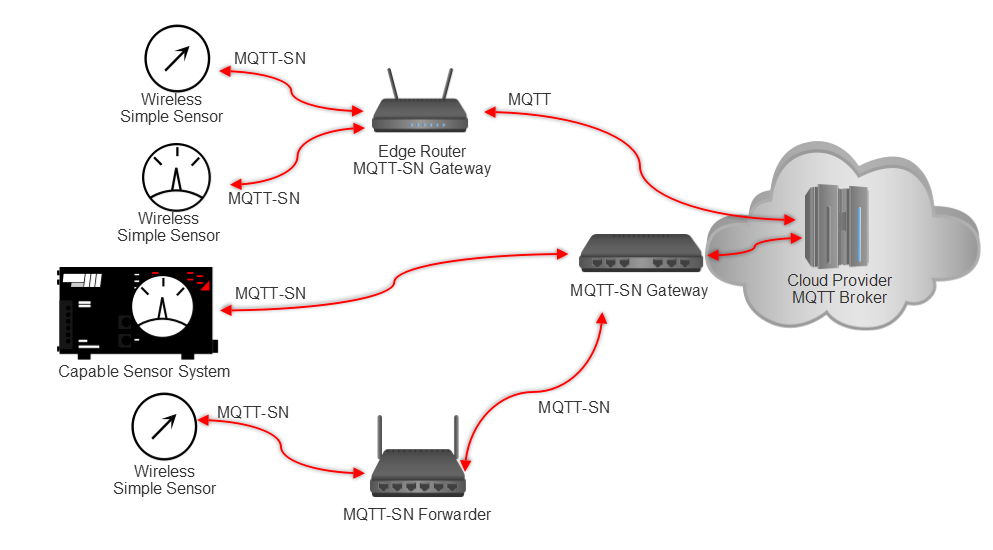
\includegraphics[scale=.35]{15a80880-30ad-472a-bf98-254556798207.png}}
\end{figure}
\begin{itemize}
	\item \textbf{Endpoints:} Los distintos sensores o dispositivos.
	\item \textbf{Gateways - Puertas de enlace:} Son los responsables de convertir MQTT-SN a MQTT para enviarlo al router. Se pueden tener retransmisores y repetidores, que permiten que llegue más lejos la señal cuando se encuentran en lugares remotos.
\end{itemize}

Los gateways/routers envían periódicamente mensajes broadcast (ADVERTISE) informando de que están disponibles, de esta manera los clientes pueden buscar los gateways a los que se pueden conectar con SEARCHGW, y estos les responderán con GWAINFO con la información de puerta de enlace.
\begin{itemize}
	\item \textbf{ADVERTISE:} Se transmite periódicamente desde una puerta de enlace para anunciar su presencia.
	\item \textbf{SEARCHGW:} Emitido por un cliente cuando busca una puerta de enlace en particular. Parte del mensaje es un parámetro de radio, que indica cuántos saltos debe seguir el mensaje SEARCHGW en una topología de red.
	\item \textbf{GWINFO:} Esta es la respuesta de las puertas de enlace al recibir un mensaje SEARCHGW. Contiene el ID y la dirección de la puerta de enlace, que solo se transmite cuando SEARCHGW se envía desde un cliente.
\end{itemize}

\subsection{Diferencias con el MQTT}
\begin{itemize}
	\item Hay tres mensajes CONNECT en MQTT-SN frente a uno en MQTT, los dos adicionales se utilizan para transportar además el tema o el mensaje explícitamente.
	\item MQTT-SN se puede ejecutar en un medio simplificado y UDP.
	\item Los nombres de los temas se reemplazan por mensajes de ID de tema cortos de dos bytes de longitud. Esto es para ayudar con las limitaciones de ancho de banda en las redes inalámbricas.
	\item Los ID de tema predeterminados y los nombres cortos de tema se pueden usar sin ningún registro. Para utilizar esta función, tanto el cliente como el servidor deben utilizar el mismo ID de tema. Los nombres breves de los temas son lo suficientemente cortos como para incluirse en el mensaje PUBLISH.
	\item Se introduce un procedimiento de descubrimiento para ayudar a los clientes y permitirles encontrar las direcciones de red de servidores y puertas de enlace. Pueden existir varias puertas de enlace en la topología y se pueden utilizar para compartir la carga de la comunicación con los clientes.
\end{itemize}

\section{CoAP (Constrained Application Protocol) - Protocolo de Aplicación Restringida}
Es un estándar del IETF, está pensado para facilitar la conexión entre dos máquinas punto a punto.

El broker no existe como tal, sino que para conectarte a un servidor necesita conocer su dirección física. Una vez establecida la conexión es hasta 64 veces mejor que su equivalente con HTTP y software similar.
\begin{figure}[H]
	\ffigbox[\FBwidth]
	{\caption{Estructura CoAP}}
	{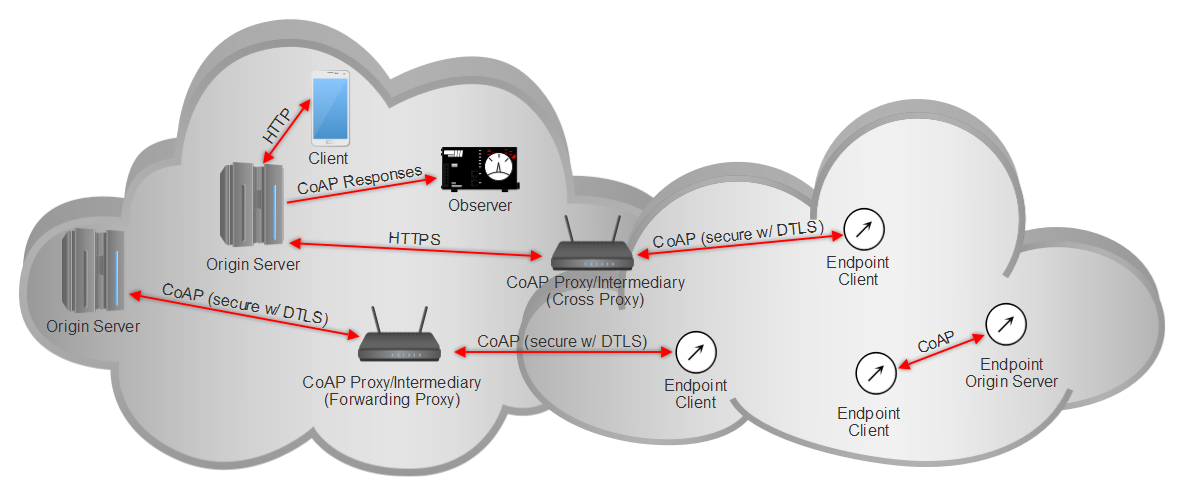
\includegraphics[scale=.35]{79e6a27f-bae5-4c7b-963a-dcd46c9e26f1.png}}
\end{figure}
\pagebreak
\subsection{Requisitos a satisfacer}
\begin{itemize}
	\item Debe tener una complejidad adecuada que se tienen en una red IoT, con baja capacidad de procesamiento y una RAM muy limitada. Memoria hasta 256 K y RAM de 12 K. Reduciendo la sobrecarga de los mensajes de HTTP, pero con un método de direccionamiento exactamente igual al de HTTP.
	\item Es necesario un mecanismo que permita gestionar la caché de solicitudes de recursos recientes, para optimizar.
	\item Tiene que implementar peticiones post, get, put y delete, de manera que permita facilitar y automatizar la creación, eliminación, lectura y actualización de un dispositivo, canal o recursos.
	\item Cada dispositivo debe tener su URI, un identificador único de recurso, similar al de URL.
	\item Periodos de latencias muy bajos.
	\item Tiene que trabajar sobre UDP, para aligerar el protocolo.
\end{itemize}

\subsection{Diferencias con MQTT}
\begin{itemize}
	\item No hay como tal broker en CoAP de manera general, pero se podría tener un observador en el medio que gestione las publicaciones.
	\item Es más ligero CoAP.
	\item Se pueden referenciar los recursos como si fuera una URI, para esto se necesita un resolvedor.
	\item El intercambio de mensajes es totalmente asíncrono.
\end{itemize}

\subsection{Mecanismos para la conexión}
Para que un dispositivo se conecte a un sensor, se debe realizar una petición directa al sensor.

Se utiliza el protocolo coap (coap://) en vez de http, con un nombre de URL que represente a los dispositivos (myhome.in:5683), una subdirección dentro de la URL para indicar el dispositivo (nest\_livingroom) y por último el nombre del parámetro de control del dispositivo (temp). Este último se podría completar con las distintas peticiones get, put, post o delete, que nos devuelven los datos o el código de error correspondiente (los códigos están reducidos). $$\text{coap://myhome.in:5683/nest\_livingroom/temp}$$

\subsection{Características}
\begin{itemize}
	\item Similar a HTTP, lo que cambia es el protocolo, se utiliza uno que produce muy poco tráfico.
	\item Protocolos sin conexión.
	\item Seguridad a través de DTLS en lugar de TLS en una transmisión HTTP normal.
	\item Intercambios de mensajes COMPLETAMENTE asincrónicos.
	\item Diseño liviano y requisitos de recursos y baja sobrecarga de encabezado.
	\item Soporte para URI y tipos de contenido.
	\item Basado en UDP.
	\item Un mapeo HTTP sin estado que permite a proxies enlazarse con sesiones HTTP
\end{itemize}

\subsection{Actores principales}
\begin{itemize}
	\item \textbf{Endpoints:} Son los sensores o dispositivos IoT que proporcionan información.
	\item \textbf{Proxies:} Nos permite conectar los endpoints a la red, funcionan como intermediarios de los mensajes, reciben CoAP y puede salir otro formato para los servidores.
	\item \textbf{Servidor CoAP:} Es al que nos conectamos cuando queremos obtener la información de los sensores.
	\item \textbf{Observador:} Elemento que se puede utilizar como si fuera un broker de MQTT.
	      \begin{figure}[H]
		      \ffigbox[\FBwidth]
		      {\caption{CoAP Observer}}
		      {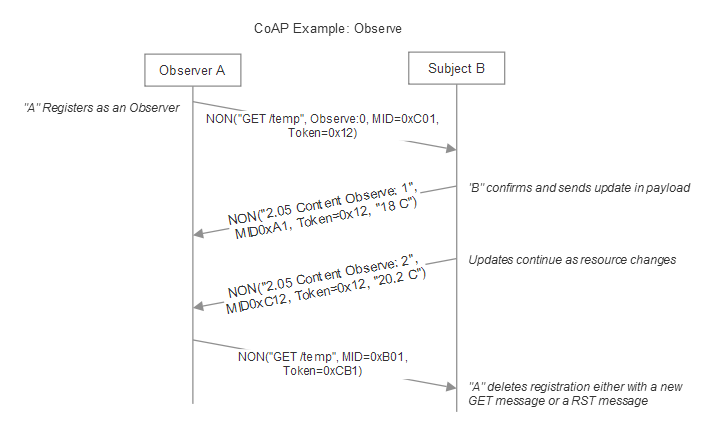
\includegraphics[scale=.48]{2a2f42a1-0813-4e84-a244-72e6f2667ba8.png}}
	      \end{figure}


\end{itemize}

\textbf{DTLS} es el protocolo de comunicación seguro que se monta sobre CoAP, da una capa de seguridad a UDP sobre los mensajes en transmisiones punto a punto.

\subsection{Tipos de mensajes}
\begin{figure}[H]
	\ffigbox[\FBwidth]
	{\caption{CoAP Messages}}
	{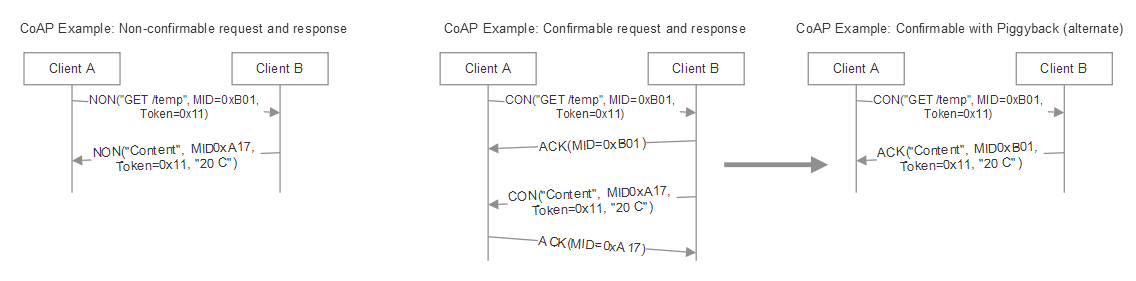
\includegraphics[scale=.48]{d5c42d4c-400c-4d55-9eea-96fc5bedf353.png}}
\end{figure}

Todos los mensajes tienen un MID (message ID) y un Token, es un código que nos da en algún momento el servidor (representa nuestros datos propios) y se utiliza para indicar quienes somos, así nos puede reconocer.

\begin{itemize}
	\item \textbf{CON - Confirmable:} Requiere un ACK. Si se envía un mensaje CON, se debe recibir un ACK dentro de un intervalo de tiempo aleatorio entre ACK\_TIMEOUT y este valor multiplicado por un valor aleatorio. Si no se recibe el ACK, el remitente transmite el mensaje CON una y otra vez a intervalos que aumentan exponencialmente hasta que recibe le ACK o un RST.
	      \begin{itemize}
		      \item El A manda CON get \/temp con un token.
		      \item El B envía un mensaje ACK al A.
		      \item El B manda CON con el contenido solicitado.
		      \item El A confirma la recepción con un ACK.
	      \end{itemize}
	\item \textbf{NON: No-confirmable:} No requiere un ACK. Esencialmente un mensaje o transmisión de disparar y olvidar.
	      \begin{itemize}
		      \item El cliente A manda un mensaje NON para get \/temp, con un token para identificarme.
		      \item El cliente B lo recibe y envía al Cliente A el contenido solicitado con el token que le envió A, para que sepa que es suyo.
	      \end{itemize}
	\item \textbf{ACK - Reconocimiento:} Reconoce mensajes CON. El mensaje ACK puede combinarse con otros datos.

	\item \textbf{RST - Reseteo:} Indica que se ha recibido un mensaje CON, pero falta el contexto. El mensaje RST puede combinarse con otros datos.
\end{itemize}

\textbf{Simétrico} ambos extremos de la comunicación tienen que ser capaces de proporcionar los mismos mensajes en la comunicación, la comunicación entre ambos nodos se realiza de la misma manera, sin embargo \textbf{asimétrico} cada uno se comporta de una manera distinta cuando se comunican.

\chapter{Tema 6: Microservicios para la gestión de nubes de dispositivos IoT}
\section{Microservicio}
Es un servicio que está disponible en la plataforma IoT y como su nombre indica (micro) proporciona una capacidad específica que necesitamos y es accesible mediante una API.

\textbf{Cohesión:} Número distinto de responsabilidades que tiene un componente.

Un microservicio es un componente que tiene vida independiente, aunque se integre en un sistema complejo puede funcionar de manera independiente.

Es micro porque esta clase de servicios tienen un conjunto de responsabilidades pequeño, porque lo que buscamos es que se puedan utilizar en multitud de entornos, así son más generales. Por ejemplo, se utilizan para gestionar sensores, solamente para recibir las mediciones de los sensores de la red, o gestionar dispositivos, para ver en qué estado están o regístralos.

Son neutrales en cuanto al lenguaje de programación, cada microservicio puede estar en uno distinto mientras se comuniquen mediante la API REST.

Al ser partes pequeñas y con función especifica pueden ser lanzados rápida y frecuentemente.

\section{Interfaz API ReST}
Es un servicio/API que es independiente del estado en el que se encuentra el servidor. (CoAP es un ejemplo de una implementación de API ReST)

Mecanismo que se utiliza para exponer distintos microservicios. Sirve para implementar o hacer visibles las funcionalidades o capacidades que exponen las distintas partes de la plataforma/nube IoT.

Las API RESTful son útiles para funciones de soporte y utilidades que no necesitan conectividad o ser en tiempo real.

Aunque normalmente lo utilizan programas y aplicaciones ascendentes, los dispositivos descendentes también pueden acceder a estas API cuando sea necesario. Proporcionará una serie de métodos disponibles para los usuarios del microservicio.


\section{Gestión de una red de dispositivos IoT}
Para gestionar el gran volumen de información que se mueve, lo que se necesita es que los elementos de la nube IoT sean elásticos, es decir que a nivel tecnológico se pueda pasar de proporcionar servicio a un centenar de dispositivos a centenares de miles de dispositivos.

Otra manera para flexibilizar el despliegue de microservicios es que tenga su propio almacén de datos, así se pueden hacer consultas más refinadas.

Es fundamental tener servicios muy atómicos que se puedan transportar muy fácilmente (llevar de una parte a otra) y que se puedan replicar de manera eficiente en muchos servidores para trabajar de manera colaborativa.

En contenedores se verá cómo se despliega.

Los microservicios deben ser configurables de manera automática, es decir con archivos externos de configuración con toda la información necesaria para crear distintas instancias del microservicio.

\section{Áreas de los Microservicios y su tipo}
\begin{itemize}
	\item \textbf{Gestión de Dispositivos - Device Microservice}, se encarga de registrar, de registrar y conocer el estado de los dispositivos para transmitirla.
	\item \textbf{Ingestión de telemétrica - Ingestion Event Hub}, recepción de mensajes de los dispositivos que tengamos distribuidos por el mundo. Gestiona grandes cantidades de datos.
	\item \textbf{Transformación y Almacenamiento - Event Relational Store}.
	\item \textbf{Estado y Notificaciones - Alarm Event Hub}.
	\item \textbf{Analíticas y Visualización de Datos - Reference Data Microservice}.
\end{itemize}


\section{Características}
\begin{description}
	\item[Autónomos] Capaz de existir independientemente de otros componentes de la plataforma IoT, responder, reaccionar o desarrollase independientemente del todo. Que se pueda tener funciones sin requerir el todo y estos componentes se pueden poner a ejecutar de manera aislada.
	\item[Aislados] Capaz de ejecutarse aisladamente de los demás componentes, pudiéndose ejecutar en diferentes lugares y en diferentes momentos.
	      \pagebreak
	\item[Elástico] Cuando gestionando los recursos de manera razonable es capaz de proporcionar servicio a centenares de usuarios y a centenares de miles de usuarios, es capaz de estirarse para dar servicio a más usuarios sin necesidad de desarrollo adicional, solo replicando el microservicio en contenedores y servidores
	\item[Resiliente] Capaz de mantenerse en funcionamiento después de un error, no se queda bloqueada, se debe poder recuperar.
	\item[Responsive] Debe proporcionar una respuesta rápida y eficiente por muchos usuarios que se tenga.
	\item[Orientado a mensaje] Disponible a partir de una interfaz HTTP, que los datos se transferirán mediante una llamada CoAP, HTTP o similar, y los datos están guardados en un objeto (de una manera más rica) como JSON o binario, de manera que los sistemas separados en una red estén conectados.

	      Si quiero acceder a un método de un microservicio haré una petición get, post, put o delete, si está en una nube mediante HTTP y si es un dispositivo con la nube mediante CoAP o MQTT.

	\item[Programable] Un plan de tareas que se realizan con el fin de lograr un resultado específico. Que estas funcionalidades de la API se puedan acceder desde un navegador o por medio de otras aplicaciones. Esta programación en un microservicio se hace mediante un protocolo de red.
	\item[Configurable] Diseñado para poderse adaptar a diferentes configuraciones específicas, que se tiene que adaptar a las distintas posibles configuraciones de despliegue, hacer que sea más fácil realizar estas configuraciones. Diseñado para poderse adaptar a diferentes configuraciones específicas o para algún propósito específico.
	\item[Automatizado] Tener controles que permitan que algo funcione o suceda sin ser controlado directamente por una persona.
\end{description}

\section{Arquitectura de Microservicios}

El principio básico para el desarrollo de una arquitectura de servicios en la nube, como es el IoT, consiste en la separación de intereses, siguiendo un principio de diseño que permite separar la implementación de todo un sistema complejo en distintas capas, donde cada capa tiene su ámbito o foco de actuación.

Esa separación se logra mediante el encapsulamiento e interfaces bien definidas, que es lo que buscamos con los microservicios.
Este tipo de encapsulamiento se debe hacer en las 5 áreas que se describen arriba.

En función de la separación de los intereses hay distintos tipos de arquitecturas.

\subsection{Solución monolítica}
Aquellas que se implementan como un gran cuerpo con todo el código y se necesita tenerlo completo para utilizar el sistema.

No se encuentra divida en partes más pequeñas (como podrían ser microservicios) para obtener solo lo que nos interesa.

Esto hace que sea muy difícil de mantener y evolucionar, todo está muy acoplado entre sí.

\subsection{Arquitectura en capas}
Se establecen unas capas según las funcionalidades e intereses.

\subsubsection{Modelo Vista Controlador}
\begin{figure}[H]
	\ffigbox[\FBwidth]
	{\caption{Arquitectura Modelo Vista Controlador}}
	{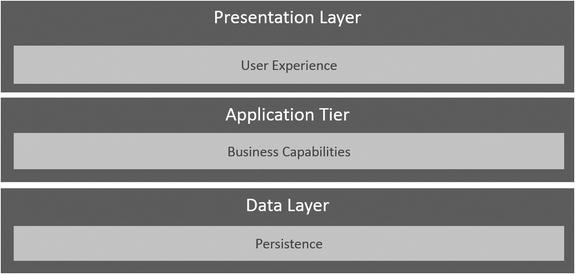
\includegraphics[scale=.8]{9781484212769_Fig03-01.jpg}}
\end{figure}
\begin{itemize}
	\item \textbf{Presentación}, la de interfaz de usuario, lo que se muestra al usuario e interactúa.
	\item \textbf{Aplicación}, tiene toda la lógica de negocio.

	      Es una capa monolítica si se quiere cambiar algo de esta capa hay que reinstalar toda la capa por completo, como si fuera un monolito.

	\item \textbf{Persistencia}, donde se produce el almacenamiento y consulta de datos.
\end{itemize}
\pagebreak
\subsubsection{Aplicaciones normales}

Se tiene una evolución muy superior que MVC, consisten en proporcionar diferentes interfaces de usuario mediante contratos o servicios web.

\begin{figure}[H]
	\ffigbox[\FBwidth]
	{\caption{Arquitectura en capas}}
	{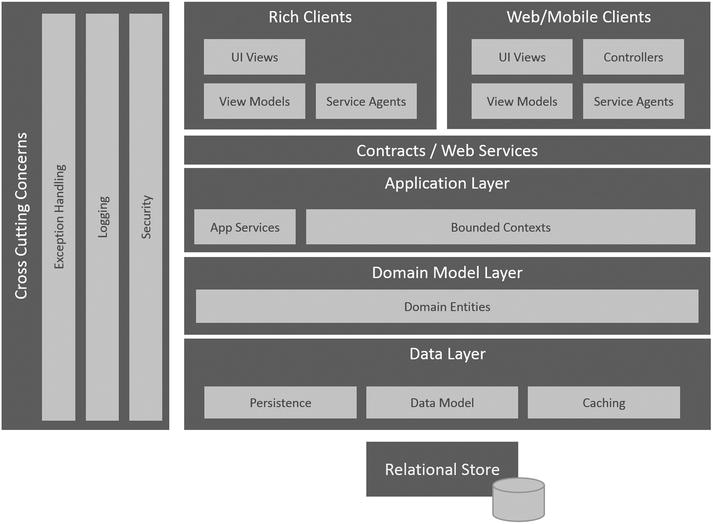
\includegraphics[scale=.8]{9781484212769_Fig03-02.jpg}}
\end{figure}

\begin{itemize}
	\item \textbf{Clientes móvil/web}: Se pueden conectar vía móvil, tablet, web, etc.
	\item \textbf{Clientes ricos}: Como puede ser el que se puede acceder desde un computador de escritorio, en el que se puede proporcionar y acceder a mucha más información.
	\item \textbf{Contratos y Servicios web}: Para controlar las diferentes interfaces se utiliza SOAP o REST.

	      \textbf{SOAP} es un protocolo específico que se gestiona de manera independiente a HTTP y tiene otros estándares adicionales para publicar servicios complejos en internet, que permite implementar más seguridad o atomicidad de las operaciones. Emplea XML.

	      \textbf{REST} es un estilo arquitectónico para exponer servicios web en internet mediante HTTP y que nos permite más tipos. Emplea XML o JSON, permite más tipos de protocolos.

	\item \textbf{Capa de dominio:} Es donde se tienen las reglas de negocio.
	\item \textbf{Capa de aplicación}: Se coreografían las reglas de negocio.
	\item \textbf{Capa de almacenamiento}: Se tienen las distintas operaciones de gestión de los datos, desde la gestión física de datos, hasta el modelo de datos y el cacheo.
\end{itemize}

\pagebreak
\subsection{Arquitectura de Microservicios}
En las arquitecturas de microservicios las 3 capas (Presentación, Aplicación y Persistencia) están separadas en diferentes nodos que pueden trabajar de manera independiente y luego hay servicios que coreografían las peticiones para realizar las operaciones de manera atómica.

\begin{figure}[H]
	\ffigbox[\FBwidth]
	{\caption{Arquitectura de Microservicios}}
	{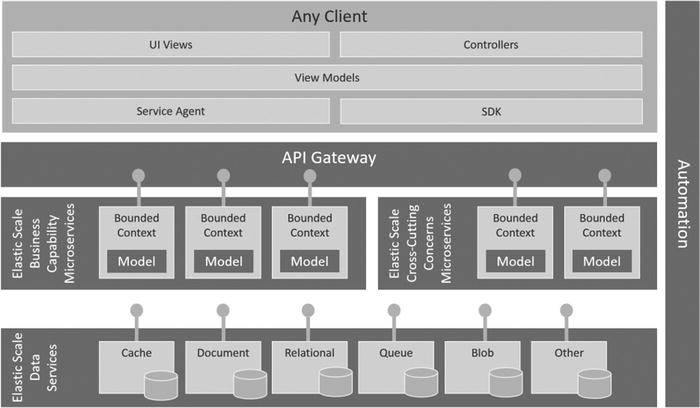
\includegraphics[scale=.8]{9781484212769_Fig03-03.jpg}}
\end{figure}
\vspace{-0.5cm}
La capa de aplicación está formada por microservicios que se coordinan con una API que hace de coreografiador según las peticiones que recibe de la WebApp.

Cuando se recibe una petición de la WebApp se pasa a la API (coreografiador) que se encarga de pasarla al microservicio correcto para realizar lo solicitado, cada microservicio posee sus propios datos con su propio gestor de bases de datos.

Incluso un mismo microservicio según la configuración que le demos puede utilizar un gestor de bases de datos u otro.

\subsection{Ventajas de las Arquitecturas de Microservicios}
\begin{itemize}
	\item Mejor escalabilidad del desarrollo, cada microservicio se centra en una cuestión, de esta manera el trabajo de desarrollo se puede dividir entre distintos equipos de desarrollo y que sean más diversos.
	\item Mayor velocidad de desarrollo, al haber más equipos que trabajen en paralelo.
	\item Apoya la modernización iterativa o incremental.
	\item Aprovecha el moderno ecosistema de desarrollo de software (nube, contenedores, DevOps, sin servidor), nos permite desplegar en un nodo independiente cada uno de estos microservicios de esta manera se da servicio a más sistemas.
	\item Admite escalado horizontal y granulado.
	\item Pone poca complejidad cognitiva en la cabeza del desarrollador gracias a su tamaño más pequeño.
\end{itemize}

\section{Elementos de los Microservicios}

\begin{figure}[H]
	\ffigbox[\FBwidth]
	{\caption{Elementos de un Microservicio}}
	{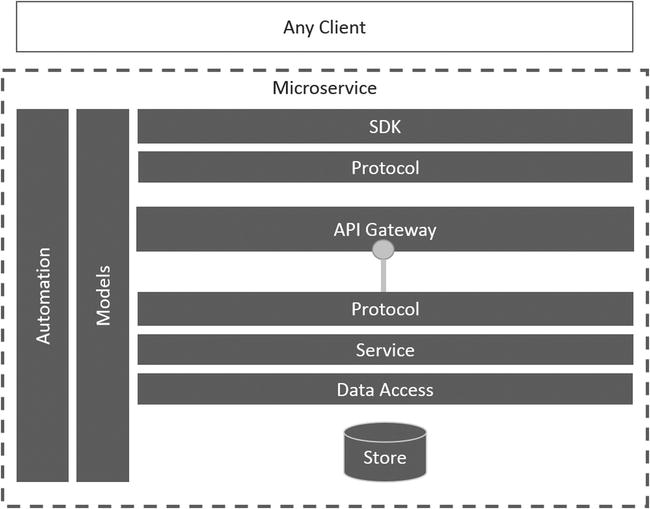
\includegraphics[scale=.8]{9781484212769_Fig03-04.jpg}}
\end{figure}

\begin{itemize}
	\item \textbf{Capa de modelos:} Tiene su propio modelo de datos que es la estructura que deben tener los datos que entran y salen de nuestros microservicios. En la práctica el modelo de datos es agnóstico, independiente.
	\item \textbf{Capa de SDK - Software Development Kit:} Conjunto de herramientas y librerías que se utilizan para desarrollar código, incluye funciones que realizan las llamadas a la API ReST para facilitarnos interactuar con ellas de manera que no haga falta que lo hagamos nosotros.
	\item Nuestros microservicios van a utilizar comunicación HTTP, por lo tanto, dentro de sus elementos se encuentran las distintas peticiones.
	      \begin{itemize}
		      \item \textbf{GET - Leer}: Puede hacerse de manera simple, mediante la URL con el ID a consultar, o más compleja mediante el uso de una interrogación e igual, para determinar los parámetros y debe ser capaz de trabajar con estos.

		            GET http://myapi.looksfamiliar.com/profiles/user/id/99999

		            GET http://myapi.looksfamiliar.com/profiles?location=Massachusetts

		      \item \textbf{POST - Crear}: Peticiones que nos permiten crear elementos, los parámetros se pasan con una estructura determinada como JSON

		            \{ \"id" : "99999", "first" : "Bob", "last" : "Familiar" \}

		            POST http://myapi.looksfamiliar.com/profiles/user

		      \item \textbf{PUT - Sustituir o actualizar}
		      \item \textbf{PATCH - Modificar Parcialmente}
		      \item \textbf{DELETE - Borrar}
	      \end{itemize}
	\item \textbf{Protocolo:} Puede ser de dos tipos ReST o SOAP.
	      \begin{table}[H]
		      \begin{tabular}{l|c|c|}
			      \cline{2-3}
			        & \textbf{SOAP/WSPL}                   & \textbf{ReST}                \\ \hline
			      \multicolumn{1}{|l|}{\textbf{Estilo}}
			        & Protocolo                            & Arquitectónico               \\ \hline
			      \multicolumn{1}{|l|}{\textbf{Foco}}
			        & \begin{tabular}[c]{@{}c@{}}Orientado a la funcionalidad\\ - Hacer Transacciones\end{tabular}           & \begin{tabular}[c]{@{}c@{}}Orientado a datos - \\ Acceder a los datos de un recurso\end{tabular}   \\ \hline
			      \multicolumn{1}{|l|}{\textbf{\begin{tabular}[c]{@{}l@{}}Formato \\ de Datos\end{tabular}}}
			        & XML                                  & Texto, JSON, HTML, XML       \\ \hline
			      \multicolumn{1}{|l|}{\textbf{Seguridad}}
			        & WS-Security -\textgreater SSL        & TLS y SSL -\textgreater HTTP \\ \hline
			      \multicolumn{1}{|l|}{\textbf{\begin{tabular}[c]{@{}l@{}}Ancho \\ de banda\end{tabular}}} &
			      \begin{tabular}[c]{@{}c@{}}Requiere más al usar XML y ser un \\ protocolo, tiene su propia secuencia de \\ negociación de mensajes, más tráfico\end{tabular} & Requiere menos \\ \hline
			      \multicolumn{1}{|l|}{\textbf{Cache}}
			        & No se puede gestionar                & Puede gestionar caché        \\ \hline
			      \multicolumn{1}{|l|}{\textbf{\begin{tabular}[c]{@{}l@{}}Contrato \\ de datos\end{tabular}}}
			        & Necesito conocer la Clase del Objeto & \begin{tabular}[c]{@{}c@{}}No tiene por qué ser conocido \\ el tipo de datos previamente\end{tabular}   \\ \hline
			      \multicolumn{1}{|l|}{\textbf{Atomicidad}}
			        & Si                                   & No                           \\ \hline
		      \end{tabular}
		      \caption{Diferencias entre SOAP y ReST}
	      \end{table}
	\item \textbf{API Gateway}
	\item \textbf{Capa de Servicio}: Es donde realmente se implementa el funcionamiento, el código que tenemos que utilizar para implementar los métodos que se exponen sobre la API. Actúa con la capa de acceso a datos para gestionar los datos en persistencia.
	\item \textbf{Capa de Acceso a Datos}: Gestión de la persistencia de los datos y las caches. Interfaces para acceder a los datos.
	\item \textbf{Capa de Automatización}: Es la que permite configurar mediante una secuencia de script, lanzar y ejecutar las distintas instancias de los microservicios mediante tecnología como contenedores, todo de manera automatizada.
\end{itemize}

\section{Características Importantes de una Arquitectura de Microservicios}
\begin{figure}[H]
	\ffigbox[\FBwidth]
	{\caption{Arquitectura de Microservicios II}}
	{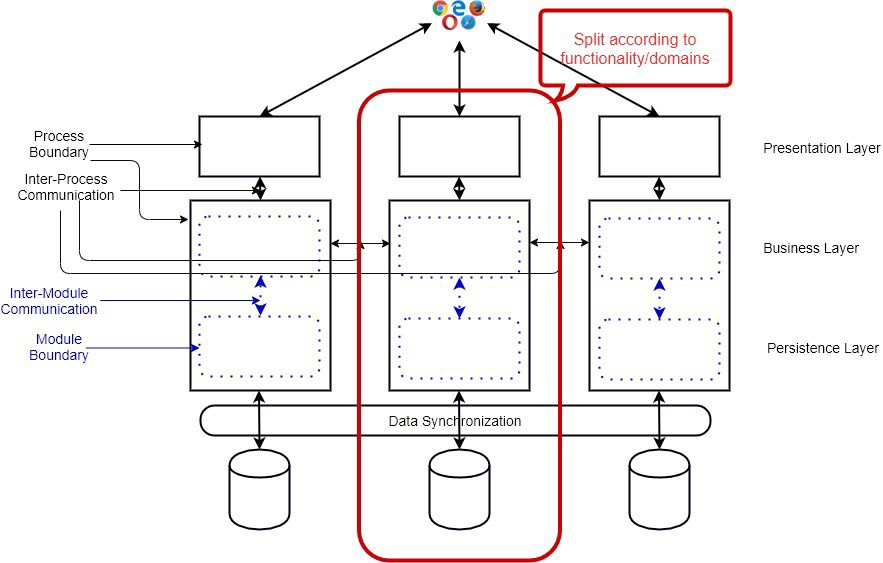
\includegraphics[scale=.3]{0_W5T2tfcKgudQZYnu.jpeg}}
\end{figure}

Toda aplicación se divide en procesos separados, donde cada proceso tiene distintos módulos internos, de manera que cada uno es un pequeño monolito que puede trabajar de  manera independiente.

Para desarrollar estas arquitecturas podemos utilizar distintos patrones de diseño, que son parejas de problema-solución software, donde la solución viene dada como una guía de cómo resolver ese problema específico.

Algunos patrones de diseño para microservicios son:

\subsection{Base de datos por microservicio}
\begin{figure}[H]
	\ffigbox[\FBwidth]
	{\caption{Database per Microservice}}
	{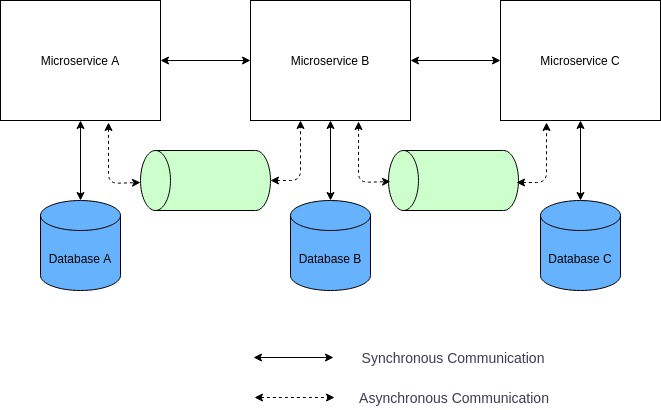
\includegraphics[scale=.3]{1_WWJQH50jxgrqh-ABFRQuzQ.jpeg}}
\end{figure}

Un único repositorio de datos para cada microservicio se trata de reducir el acoplamiento entre ellos, la dependencia.

El problema es como permitir que los distintos microservicios intercambien información entre sí, se comunicarían de manera asíncrona, para solventar esto se usa lo siguiente.

\subsection{Abastecimiento de eventos}
\begin{figure}[H]
	\ffigbox[\FBwidth]
	{\caption{Event Sourcing}}
	{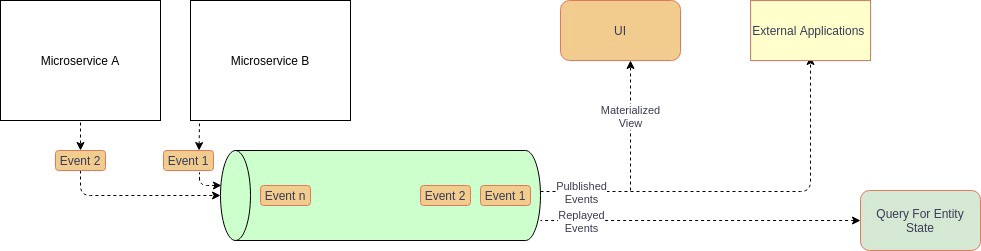
\includegraphics[scale=.3]{1_tRDaroNg_GnGdCZDFxLFKQ.jpeg}}
\end{figure}

Para que intercambien información necesitamos implementar un coreografiador que sea capaz de almacenar los distintos eventos, y cuando hemos completado estos eventos le damos la información a los elementos de la interfaz de usuario para identificar que la operación se ha realizado correctamente.

Se meten las distintas peticiones en una cola de mensajes síncrona, de tal manera que se ejecutan los eventos en orden, de manera que cuando se ejecutan con éxito, se asegura que se haya ejecutado convenientemente.

En caso de que un evento provoque una situación de error, todos los anteriores se deshacen para evitar problemas de atomicidad de estos elementos.
\begin{itemize}
	\item \textbf{Pros:} Proporciona soluciones atómicas bien definidas y se tiene un registro de las peticiones de los microservicios, incluso un registro por cada microservicio. Se realiza mediante eventos y no compartiendo datos o estructura.
	\item \textbf{Contras:} Realizar esas coreografías es complejo y requiere un almacén adicional para las peticiones y estado antes y después de cada evento,  para poder ante cualquier problema volver al estado anterior.
\end{itemize}

\subsection{Backends para Frontends (BFF)}
\begin{figure}[H]
	\ffigbox[\FBwidth]
	{\caption{Backends for Frontends}}
	{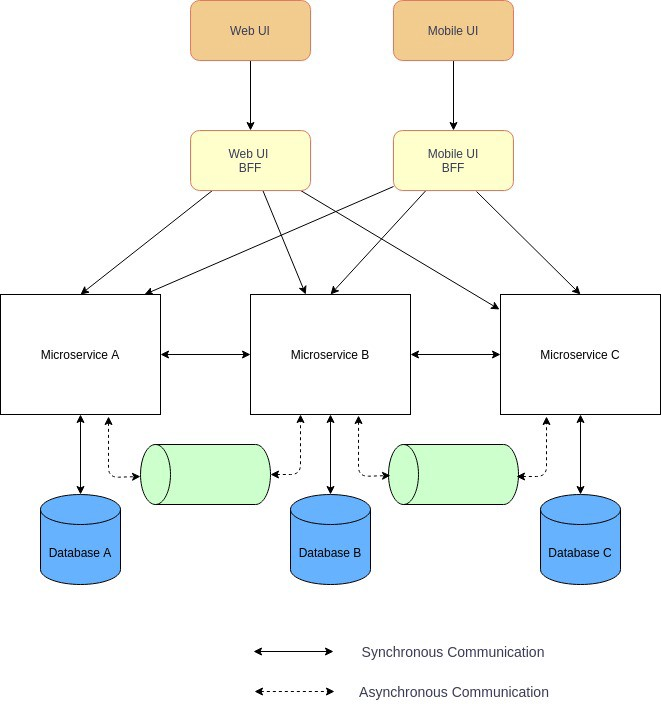
\includegraphics[scale=.3]{1_FCZRcAuSLhrNOjcq1zYXDw.jpeg}}
\end{figure}

Como se tienen distintas interfaces que tienen distintos componentes de interfaz visual, se utiliza un orquestador distinto para los distintos tipos de interfaces de usuario (web/mobile), se gestionan los microservicios de manera distinta para que se adapten mejor a estas.

Por ejemplo, el móvil es menos seguro y usa menos recursos, por lo que recibe datos menos ricos.

Al estar separadas se exponen distintas funcionalidades, por lo que se puede proteger para aquellas más vulnerables.

Se gestiona un backends para cada interfaz cuenta con su orquestador/coreografiador.

\begin{itemize}
	\item \textbf{Contras:} El problema es que se puede producir lógica duplicada, que resulta problemático a la hora de realizar las pruebas y corregir los errores.

	      Hay muchas posibles interfaces lo que hace que se vuelva más complejo, al haber tanta variedad de dispositivos, necesidades por cubrir y requisitos que satisfacer.
\end{itemize}
\pagebreak
\section{Preguntas Test 3}
\begin{enumerate}
	\item Indique el orden CORRECTO de los eventos para la verificación periódica de la conexión de los clientes en el protocolo MQTT:

	      1 - El publicador recibe del broker la confirmación de recepción del PINGREQ

	      2 - El publicador A publica un mensaje a través del broker

	      3 - El publicador A detecta que ha pasado el tiempo máximo entre mensajes

	      4 - El publicador envía un mensaje PINGREQ al broker

	      Seleccione una:

	      a. 2, 3, 4, 1

	\item Seleccione la respuesta CORRECTA con respecto a las diferencias entre MQTT y MQTT-SN. Seleccione una:

	      b. En MQTT-SN, se introduce un procedimiento de descubrimiento para ayudar a los clientes y permitirles encontrar las direcciones de red de servidores y puertas de enlace.

	\item Seleccione la afirmación INCORRECTA con respecto a las desventajas de las arquitecturas de microservicio. Seleccione una:

	      d. La complejidad pasa de la infraestructura al código.

	\item Seleccione la afirmación CORRECTA con respecto a los elementos de un microservicio. Seleccione una:

	      b. Los modelos definen la estructura de los datos a medida que entran y salen de un microservicio.

	\item Seleccione la respuesta INCORRECTA con respecto a las diferencias entre el Constrained Application Protocol (CoAP) y MQTT.
	      Seleccione una:

	      a. MQTT utiliza el modelo de comunicación solicitud-respuesta.

	\item Seleccione la respuesta CORRECTA con respecto a los mensajes del Protocolo de aplicación restringida (CoAP). Seleccione una:

	      d. Si se envía un mensaje CON, se debe recibir un ACK dentro de un intervalo de tiempo aleatorio entre ACK\_TIMEOUT y (ACK\_TIMEOUT * ACK\_RANDOM \_FACTOR).

	\item Seleccione la respuesta CORRECTA con respecto a los niveles de calidad de servicio en el protocolo MQTT.	Seleccione una:

	      a. El modo QoS-1 garantizará la entrega del mensaje al menos una vez al receptor.

	\item Seleccione la afirmación INCORRECTA con respecto a las características de los microservicios. Seleccione una:

	      c. El concepto de "micro" en microservicio se refiere al tamaño del componente de software.

	\item Seleccione la afirmación CORRECTA con respecto a los beneficios de la base de datos por patrón de microservicio. Seleccione una:

	      d. Proporciona la propiedad completa de los datos a un servicio.
	\item Seleccione la afirmación INCORRECTA con respecto a la comparación entre REST API y SOAP / WSDL. 	Seleccione una:

	      b. REST es un protocolo, mientras que SOAP es un estilo de arquitectura.
\end{enumerate}

\chapter{Tema 7: Introducción a Contenedores}
\section{Introducción}
Es una analogía con el transporte de grandes cargas en contenedores de tamaño estándar, que les permite ser transportados fácilmente en camiones, trenes y barcos; maquinaria especializada.

Es un sistema de transporte muy estándar. Independientemente de la funcionalidad que integre queremos que sea estándar, como una caja negra.

En los proyectos debe haber alguien que se encargue de controlar los problemas en la cadena de suministros, para que se utilicen las versiones correctas y todo pueda ser desplegado y probado.
\begin{itemize}
	\item \textbf{DevOps:} Se encarga de establecer entornos que permiten la integración, prueba y despliegue automatizado, que se puede conseguir con contenedores.
\end{itemize}

Un primer enfoque para resolver los problemas anteriores es utilizar \textbf{Máquinas Virtuales}, en la que en cada una tiene sus propias librerías y son independientes, pero tenemos el problema de que hay que mantenerlas todas actualizadas y se están utilizando demasiados recursos para correr una parte de nuestros sistemas (estamos matando moscas a cañonazos).
Necesitamos un nuevo mecanismo para gestionar estas infraestructuras eficientemente.

\section{Que son los contenedores?}
En los 2000 surgieron los contenedores como ese mecanismo para gestionar las infraestructuras que necesitábamos, que son unidades estándar de software que empaquetan una aplicación que hemos desarrollado y todas sus dependencias, se ejecutan de manera aislada (muy importante para que no afecte al resto de la máquina), rápida y confiable.

\begin{itemize}
	\item \textbf{Contenedor:} Una unidad estándar de software \textbf{en ejecución}, que empaqueta el código y todas sus referencias.
	\item \textbf{Imagen:} Es el conjunto de fichero que define el contenido o lo que puede ejecutar un contenedor.
	      Una imagen de contenedor es un paquete de software ligero e independiente, que incluyen lo necesario para correr la aplicación.
\end{itemize}

La diferencia con la alternativa de máquinas virtuales es que no tenemos un hipervisor, sino un sistema operativo base y un motor que es capaz de ejecutar distintos contenedores, donde cada contenedor tiene sus dependencias, sus sistemas de configuración y el código de la aplicación a desarrollar. Es mucho más liviano un contenedor que una máquina virtual, encapsula lo que se necesita para funcionar.

Docker fue el que introdujo el término de contenedor, pero hoy en día hay más alternativas como OpenShift de Red Hat o Kubernetes de Google.

\subsection{¿Por qué son importantes los contenedores?}
\begin{itemize}
	\item Las aplicaciones que se ejecutan en un contenedor son \textbf{más seguras que sus contrapartes} que no se ejecutan en un contenedor, ya que a nivel interno utiliza el espacio de nombre de kernel de Linux, lo que nos permite crear una caja cerrada en la que el proceso del contenedor no puede interactuar con ningún otro proceso que se ejecuta en la máquina, tiene su propia memoria y disco (es una sandbox).

	\item Los contenedores \textbf{facilitan la simulación de un entorno de producción}, incluso en la computadora portátil de un desarrollador.
	      Facilita mucho la instalación y despliegue.

	\item Los operadores pueden finalmente \textbf{concentrarse en el aprovisionamiento de infraestructura y ejecutar y monitorear aplicaciones en producción}.
\end{itemize}

\subsection{Arquitectura de contenedores}
\begin{figure}[H]
	\ffigbox[\FBwidth]
	{\caption{Arquitectura de contenedores}}
	{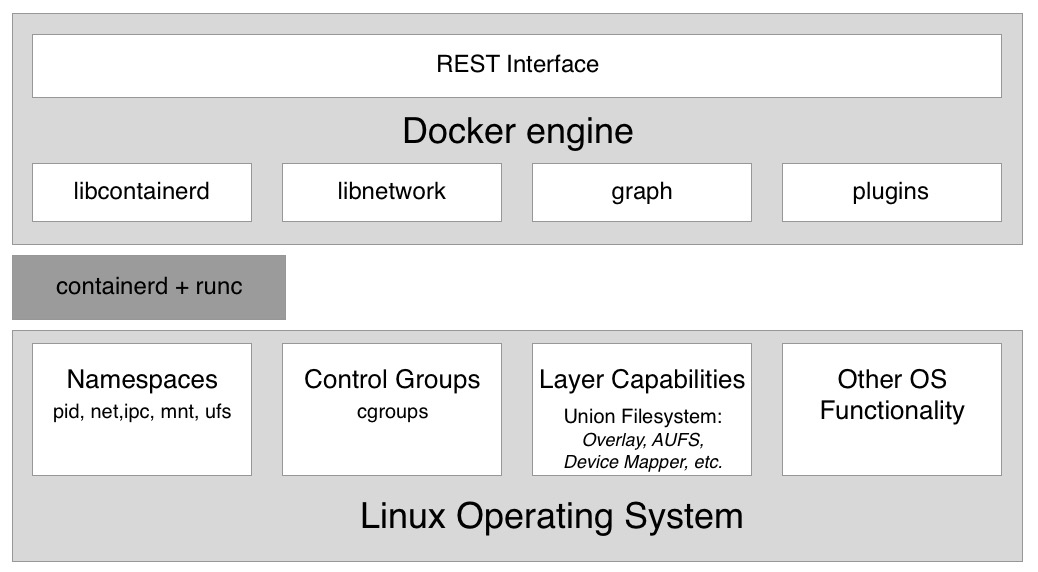
\includegraphics[scale=.4]{default.jpg}}
\end{figure}
\begin{itemize}
	\item \textbf{Sistema operativo de Linux}, lo que nos interesa son los espacios de nombres de Linux para ejecutar cada uno es un espacio y que sean independientes del resto de procesos.
	\item \textbf{Runtime engine de Docker}, se compone del demonio de contenedores containerd y el ejecutador de contenedores runc, la combinación de ambos nos da todo el tiempo de vida de un contenedor. Se coge el contenedor de una imagen y lo pone a ejecutar.
	\item \textbf{Docker engine}, proporciona la funcionalidad adicional para la gestión del contenedor en tiempo de ejecución.
\end{itemize}


\section{Creación de imágenes}
\subsection{Imagen}
En Linux todo es un archivo, de tal manera que las imágenes se gestionaran de esta manera. Es un gran fichero comprimido con su propio sistema de ficheros, que está construido en capas.

\begin{figure}[H]
	\ffigbox[\FBwidth]
	{\caption{Estructura de una imagen}}
	{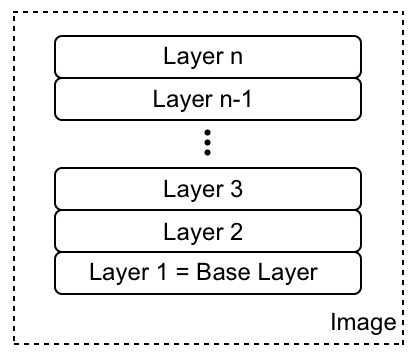
\includegraphics[scale=.5]{c4c5fd21-cc6e-49e6-b4f8-1692a5f1a561.jpg}}
\end{figure}
Cuando se tiene una imagen de un contenedor lo que se tiene es una plantilla de archivos que se va a desplegar.
\begin{itemize}
	\item La primera capa es la base, sobre esta se construyen el resto.
	\item Cada capa sobre la básica solo contiene los ficheros que vaya a añadir, eliminar o modificar con respecto a la capa anterior.
	      Se realizan las modificaciones y se empaqueta una nueva imagen hasta esta capa, que vuelvo a containerizar. Se generan imágenes de capa sobre capa.
	      \begin{itemize}
		      \item Capa 3: Añado los ficheros de datos, Add static files.
		      \item Capa 2: Añado el sistema de servidor, Add Nginx.
		      \item Capa base: El sistema operativo, Alpine Linux
	      \end{itemize}
	\item Las capas son inmutables, solo se pueden quitar eliminando los archivos de esta.
\end{itemize}


Cuando instanciamos un contenedor tenemos la capa de contenedor (sobre todas las demás), esta capa sí que es modificable para ajustar el funcionamiento de la imagen, pero el resto de las capas de la imagen son inmutables.

Si se hacen varias ejecuciones de contenedores cada uno tiene su capa de contenedor, pero estas compartirán la imagen y su estructura del sistema de ficheros.

\subsection{Docker Hub}
Es un repositorio remoto central de imágenes donde se conectan todos los Docker engine (primero se mira el repo local y si no esta se mira en Docker Hub) para obtener la imagen del container deseado.

\subsection{Copy-on-write}
Las imágenes utilizan este sistema que consiste en que si se quiere utilizar algo de otra capa se utiliza directamente de ahí, pero si se quiere modificar algo de otra capa primero se realiza una copia en nuestra capa y esta es la que se modifica.

\subsection{Docker Graph Drivers}
El copy-on-write nos permite que los controladores de grafo de Docker puedan consolidar todos los ficheros desde la última capa que lo haya instanciado hasta la raíz.

\subsection{Creación de Imágenes}
\subsubsection{Construcción de forma interactiva}
Este método consiste en ejecutar un contenedor y sobre este realizar las modificaciones que sean necesarias, en el momento que está como deseamos lo guardamos como una imagen dándole un nombre.
\begin{itemize}
	\item \textbf{docker container run -it --name ejemplo alpine /bin/sh}
	\item Hacemos desde terminal las modificaciones o instalaciones que queramos.
	\item Podemos ver con \textbf{docker container diff ejemplo} los cambios.
	\item Con \textbf{docker container commit ejemplo nombre-final} guardamos la nueva imagen.
\end{itemize}

\subsubsection{Construcción con Dockerfile}
Dockerfile es un fichero de script que nos permite describir lo que hay en la nueva imagen como la secuencia de instrucciones necesarias para generarla, luego se puede construir y ejecutar. \textbf{Ejemplo:}
\begin{lstlisting}
FROM python:2.7
RUN mkdir -p /app
WORKDIR /app
COPY ./requirements.txt /app/
RUN pip install -r requirements.txt
CMD ["python", "main.py"]
\end{lstlisting}

Cada línea constituye un nivel, el primero es la base.

\paragraph{Clausulas}
\begin{itemize}
	\item FROM es la cláusula que usa para establecer la imagen base sobre la que vamos a trabajar tiene que estar en Docker Hub, pero no tiene por qué ser un sistema operativo directamente.
	      \begin{itemize}
		      \item FROM centos:7
		      \item FROM scratch
	      \end{itemize}
	\item RUN es la cláusula que nos permite ejecutar distintos comandos sobre el sistema de la capa base. Con barra invertida (contraria a /) se puede hacer que siga en la siguiente línea.
	      \begin{itemize}
		      \item RUN apt-get update \&\& apt-get install -y wget
	      \end{itemize}
	\item COPY y ADD Permite agregar contenido a la imagen de base, COPY es sobre documentos locales y ADD nos permite además traer archivos desde un URL.
	      \begin{itemize}
		      \item COPY ./app Permite copiar en app todo lo del directorio donde se ejecuta el Docker
	      \end{itemize}
	\item WORKDIR Define el espacio de trabajo, establece el contexto de se van a realizar las ejecuciones de ahora en adelante.
	      \begin{itemize}
		      \item RUN cd /app/bin   El siguiente comando no se haría sobre bin, es necesario el WORKDIR.
		      \item WORKDIR /app/bin
		      \item RUN touch sample.txt
	      \end{itemize}
	\item CMD y ENTRYPOINT Estas cláusulas son diferentes a las anteriores, definen que va a hacer el contenedor cuando ya esté en ejecución.

	      La cabecera de los comandos se pone en ENTRYPOINT y los parámetros en CMD.
	      \begin{itemize}
		      \item ENTRYPOINT para casos en los que tienen su propia shell, como python o mariaDB, que entran en una consola propia.
		            \begin{itemize}
			            \item ENTRYPOINT["mysql"]
		            \end{itemize}
		      \item CMD dice que ejecutar, aunque puede hacerse también la entrada a shell como el ENTRYPOINT.
		            \begin{itemize}
			            \item CMD["use ipt\_data"]
		            \end{itemize}
	      \end{itemize}
\end{itemize}

\paragraph{Docker Compose}

Lo utilizaremos para ejecutar aplicaciones multiservicio/distribuidas, que tiene varios contenedores.

Es una herramienta para definir y lanzar aplicaciones distribuidas con varios contenedores con un solo comando.

Nos permite integrar todas las creaciones de contenedores dentro de un único fichero llamado docker-compose.yaml .

\textbf{Estructura:}
\begin{lstlisting}
version: "3"
services:
	nombre_contenedor:
		build: ./localizacion_del_Dockerfile
		ports:
			- "puerto_externo:puerto_interno"
		volumes:
			- volumenes de datos de almacenamiento de Datos
		links:
			- contenedor con el que estamos enlazados para sincronizarlos.
		...
\end{lstlisting}

No se tiene todo el código en un único servidor, sino que tenemos muchos de ellos, que tienen nombres que nos son amigables (identificadores).
Utilizamos un Load Balancer para balancear las peticiones que se reciben entre los diferentes servidores.

El Docker Compose nos permite automatizar las creaciones dentro de un nodo de nuestro clúster de servidores.

El \textbf{Docker Swarm} nos permite ir generando distintos nodos virtuales en los que se introducen diversos contenedores, lo que nos permite como tal lanzar la aplicación distribuida.

\subsubsection{Construcción desde un tarball}



\section{Comandos Docker}
\begin{figure}[H]
	\ffigbox[\FBwidth]
	{\caption{Estructura comando Docker}}
	{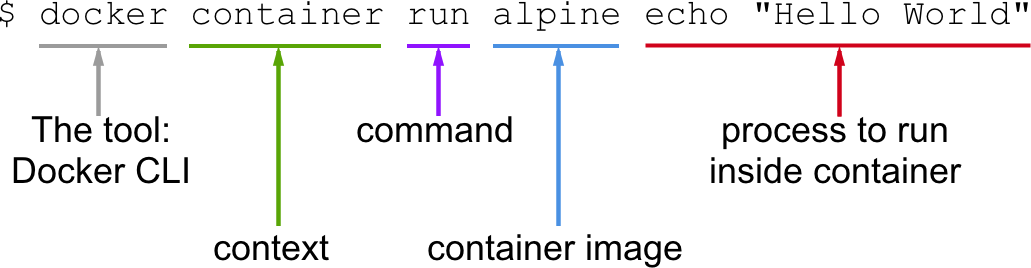
\includegraphics[scale=.3]{a18cdc15-25f8-4985-aa8d-4748d3dc2e05.png}}
\end{figure}
\begin{itemize}
	\item \textbf{docker -v}

	      Verificar versión de Docker.

	\item \textbf{docker container run alpine COMANDO}

	      Ejecutar un contenedor que corra en alpine el COMANDO.

	\item \textbf{docker container run -d alpine COMANDO}

	      -d para ejecutar un contenedor como demonio.

	\item \textbf{docker container run -it --name test alpine COMANDO}

	      --name para dar nombre al contenedor y -it para ver los mensajes de error.

	\item \textbf{docker container stop NOMBREoID}

	      Detener un contenedor.

	\item \textbf{docker container start NOMBREoID}

	      Reanudar un contenedor detenido.

	\item \textbf{docker container rm NOMBREoID}

	      Eliminar un contenedor de memoria, se puede usar -f para eliminar el contenedor este en el estado que este.

	\item \textbf{docker container ls -l / docker container ls / docker container ls -a}

	      Listar los contenedores con su ID, IMAGEN, COMANDO, CREACIÓN, ESTADO, PUERTOS y NOMBRE.
	      -l para el último, sin nada solo los en ejecución y -a para todos.

	\item \textbf{docker container ps}

	      Listar los contenedores en ejecución con su ID, IMAGEN, COMANDO, CREACIÓN, ESTADO, PUERTOS y NOMBRE.

	\item \textbf{docker container inspect NOMBREoID}

	      Muestra los detalles del contenedor en forma de JSON.

	\item \textbf{docker container exec NOMBREoID COMANDO}

	      Ejecutar comandos en un contenedor en ejecución, se puede usar -i para ejecutar el comando de forma interactiva y -t para que nos proporcione un terminal para el comando.

	\item \textbf{docker container attach NOMBREoID}

	      Ligar el contenedor a la entrada, salida y error de nuestro terminal.

	\item \textbf{docker container logs --tail 5 NOMBREoID}

	      Ver un registro de los últimos 5 procesos en ejecución en el contenedor, sin --tail 5 muestra todos.

	\item \textbf{docker container diff NOMBREoID}

	      Visualizar las diferencias que se han producido con respecto a la imagen base, A añadido, C cambiado y D borrado.

	\item \textbf{docker container commit NOMBREoID NOMBREIMAGEN}

	      Crear la imagen de un contendor en su estado actual, y le damos un nombre.

	\item \textbf{docker image ls}

	      Listar las imágenes

	\item \textbf{docker image history NOMBREoID}

	      Lista las capas sobre las que se ha construido nuestra imagen.

	\item \textbf{docker image build -t NOMBREoID}

	      Construir una imagen sin ejecutarla desde un Dockerfile.

	\item \textbf{docker image rm NOMBREoID}

	      Borra la imagen del servidor local.

	\item \textbf{docker image save -o DESTINO IMAGEN}

	      \textbf{docker image load -i ORIGEN}

	      Guardar y cargar una imagen.

	\item \textbf{docker image tag alpine:latest gnschenker/alpine:1.0}

	      \textbf{docker login -u gnschenker -p <my secret password>}

	      \textbf{docker image push gnschenker/alpine:1.0}

	      Dar etiqueta de versión a nuestra imagen, preparándola para publicarla, y subiendola a Docker Hub tras previo inicio de sesión.
\end{itemize}
\pagebreak

\section{Preguntas Test 4}
\begin{enumerate}
	\item Seleccione el comando CORRECTO que debe ejecutar cuando necesite iniciar una terminal en un contenedor en ejecución:
	      Seleccione una:

	      docker exec -it /bin/bash, docker run /bin/bash

	\item Un contenedor es:
	      Seleccione una:

	      Un método de virtualización que empaqueta el código, las configuraciones y las dependencias de una aplicación en bloques de construcción para lograr consistencia, eficiencia, productividad y control de versiones., Un paquete de software ligero, independiente y ejecutable que incluye todo lo necesario para ejecutar una aplicación.

	\item Seleccione la opción CORRECTA con respecto a los contenedores:
	      Seleccione una:

	      Las aplicaciones que se ejecutan en un contenedor son menos seguras que sus contrapartes que no se ejecutan en un contenedor., Los contenedores son bestias bastante pesadas por sí mismos, ya que todos contienen un sistema operativo completo., Los operadores de contenedores deben concentrarse en la implementación de microservicios., Los contenedores dificultan la simulación de un entorno de producción.

	\item Las diferencias entre las cláusulas ADD y COPY para la configuración de archivos de Docker son:
	      Seleccione una:

	      La cláusula ADD permite copiar archivos de URL externas.

	\item Una buena práctica para resolver los problemas de configuración de direcciones IP cuando utiliza una aplicación distribuida compuesta por una gran cantidad de microservicios es:
	      Seleccione una:

	      Servicio DNS.

	\item Las cláusulas o elementos que NO se pueden configurar en el archivo yaml docker-compose incluyen:
	      Seleccione una:

	      La respuesta correcta es: Los archivos que se agregarán a una imagen de contenedor base.

	\item Seleccione el comando CORRECTO que debe ejecutar cuando necesite ver todos los contenedores (activos o no) que se han ejecutado en una máquina:
	      Seleccione una:

	      docker container ls -l, docker ps ls -l, docker logs ls -l, docker ps

	      Enunciado de la pregunta
	\item Docker compose es una:
	      Seleccione una:

	      Herramienta para definir y ejecutar aplicaciones Docker de múltiples contenedores.

	\item Seleccione la opción CORRECTA con respecto a la arquitectura de contenedores:
	      Seleccione una:

	      El container runtime (containerd y runc) es responsable de todo el ciclo de

	\item Al configurar aplicaciones de varios contenedores con docker-compose:
	      Seleccione una:

	      Deben seguirse los tres pasos considerados en las otras opciones.
\end{enumerate}
\pagebreak

\section{Test Cuadernillo 3}

\textbf{Una opción sencilla para editar archivos de texto en la consola VM es usar}
\begin{itemize}
	\item c. nano
\end{itemize}

\textbf{El contenido de un mensaje MQTT recibido por un suscriptor puede extraerse de la variable}
\begin{itemize}
	\item b. msg.payload
\end{itemize}

\textbf{El return code (rc) que devuelve MQTT al método on\_connect para indicar que se ha conseguido establecer la conexión con éxito es}
\begin{itemize}
	\item b. 0
\end{itemize}

\textbf{La IP asignada por defecto en GCP a tu VM es}
\begin{itemize}
	\item Efímera
\end{itemize}

\textbf{Para establecer un orden correcto de despliegue de diversos dockers, usamos en docker-compose la etiqueta}
\begin{itemize}
	\item a. depends\_on
\end{itemize}

\textbf{¿Cuál es el usuario por defecto con el que inicias sesión en una nueva máquina virtual en GCP?}
\begin{itemize}
	\item c. El nombre del correo con el que te has dado de alta en GCP
\end{itemize}

\textbf{Para servir páginas desde la VM web en este curso hemos empleado}
\begin{itemize}
	\item a. apache
\end{itemize}

\textbf{La librería Python que empleamos para la conexión con un servidor MQTT es}
\begin{itemize}
	\item b. paho
\end{itemize}

\textbf{El archivo donde se especifican las características necesarias para construir y desplegar varios dockers a la vez se llama}
\begin{itemize}
	\item a. docker-compose.yml
\end{itemize}

\chapter{Recursos}
\href{https://learning.oreilly.com/playlists/5a6c045f-e39c-465e-9e7c-60dcbb12aebb}{Lista de libros de referencia}

\section{Tema 1: Arquitectura de Sistemas IoT}
\href{https://learning.oreilly.com/library/view/internet-of-things/9781788470599/a7f866bd-4ac8-47f3-a175-0f10d91a5ce2.xhtml}{Definición de Internet de las Cosas}

\href{https://learning.oreilly.com/library/view/internet-of-things/9781119456742/part04.xhtml\#part}{Aplicaciones Actuales de Internet de las Cosas}

\href{https://learning.oreilly.com/library/view/build-your-own/9781484244982/html/474034_1_En_2_Chapter.xhtml}{Arquitectura de Sistemas de Internet de las Cosas}

\section{Tema 2: Sensores y Actuadores}
\href{https://learning.oreilly.com/library/view/internet-of-things/9781788470599/d39be056-b166-476e-868e-c415e4dfa886.xhtml}{Introducción a Sensores y Actuadores} Hasta la sección 'Up to Functional examples (putting it all together)' incluida

\section{Tema 3: Sistemas operativos embebidos para Dispositivos IoT}
\href{https://learning.oreilly.com/library/view/embedded-systems-architecture/9780123821966/xhtml/CHP001.html#CHP001titl}{Introducción a los Sistemas Embebidos} Solo capítulo 1

\href{https://learning.oreilly.com/library/view/embedded-systems-architecture/9780123821966/xhtml/CHP009.html#CHP009titl}{Sistemas Operativos Embebidos} Capítulo 9

\href{https://learning.oreilly.com/library/view/embedded-systems-architecture/9780123821966/xhtml/CHP008.html#CHP008titl}{Drivers de Dispositivos} Hasta el encabezado "8.1 Example 1: Device Drivers for Interrupt Handling"

\href{https://learning.oreilly.com/library/view/embedded-systems-architecture/9780123821966/xhtml/CHP010.html#CHP010titl}{Middleware} Secciones 10.1 y 10.2

\section{Tema 5: Protocolos de comunicación de dispositivos con infraestructuras IoT}
\href{https://learning.oreilly.com/library/view/internet-of-things/9781788470599/b34f5cd8-115c-490c-b5c2-38a3a966a65a.xhtml}{Protocolos de comunicación IoT}

\section{Tema 6: Microservicios para la gestión de nubes de dispositivos IoT}
\href{https://learning.oreilly.com/library/view/microservices-iot-and/9781484212752/9781484212769_Ch02.xhtml}{¿Qué es un microservicio?} Capítulo 2 completo

\href{https://learning.oreilly.com/library/view/microservices-iot-and/9781484212752/9781484212769_Ch03.xhtml}{Arquitecturas de Microservicios} Capítulo 3 completo

\href{https://towardsdatascience.com/microservice-architecture-and-its-10-most-important-design-patterns-824952d7fa41}{Patrones de Diseño de Microservicios} Artículo completo

\section{Tema 7: Introducción a Contenedores}
\href{https://learning.oreilly.com/library/view/getting-started-with/9781838645700/fb4efc86-2e13-4f11-94be-2485878464ca.xhtml}{¿Qué son los contenedores y por qué debemos utilizarlos?}

\href{https://learning.oreilly.com/library/view/getting-started-with/9781838645700/9f8c7bb0-cd1d-4dc3-8d6b-c08ef3590c44.xhtml}{Instalar el entorno de trabajo de Dockers}

\href{https://learning.oreilly.com/library/view/getting-started-with/9781838645700/ef53b9f7-3bd4-459e-9665-a53931a3ae0a.xhtml}{Trabajando con contenedores}

\href{https://learning.oreilly.com/library/view/getting-started-with/9781838645700/dd4d8c8e-9219-412e-853a-e52ea9de9183.xhtml}{¿Qué son imágenes y cómo se crean?}

\href{https://learning.oreilly.com/library/view/getting-started-with/9781838645700/ff4d6320-c32f-481e-8269-dbd7b5a7cec5.xhtml}{Aplicaciones Multiservicio - Docker Compose}

\end{document}
